%% Преамбула TeX-файла

% 1. Стиль и язык
\documentclass[utf8x]{G7-32} % Стиль (по умолчанию будет 14pt)
\usepackage[T2A]{fontenc}
\usepackage[russian]{babel}
\setcounter{page}{4}
% Остальные стандартные настройки убраны в preamble.inc.tex.
%%==========================================%%
%% Для избежания переносов слов
\usepackage{ragged2e}
\usepackage{microtype}

\justifying
\sloppy
\tolerance=500
\hyphenpenalty=10000
\emergencystretch=3em
%%==========================================%%

% Настройки стиля ГОСТ 7-32
% Для начала определяем, хотим мы или нет, чтобы рисунки и таблицы нумеровались в пределах раздела, или нам нужна сквозная нумерация.
\EqInChapter % формулы будут нумероваться в пределах раздела
\TableInChapter % таблицы будут нумероваться в пределах раздела
\PicInChapter % рисунки будут нумероваться в пределах раздела

% Добавляем гипертекстовое оглавление в PDF
\usepackage[
bookmarks=true, colorlinks=true, unicode=true,
urlcolor=black,linkcolor=black, anchorcolor=black,
citecolor=black, menucolor=black, filecolor=black,
]{hyperref}

%Величина «красной строки»


\usepackage[tableposition=top,singlelinecheck=false]{caption}
%\usepackage{subcaption}

\DeclareCaptionLabelFormat{gostfigure}{Рисунок #2}
\DeclareCaptionLabelFormat{gosttable}{Таблица #2}
\DeclareCaptionLabelSeparator{gost}{~---~}
% Можно разбивать длинные таблицы вручную, оформляя каждую как table. В этом случае для продолжений таблицы нужно создать отдельный стиль заголовка
\DeclareCaptionLabelFormat{continued}{Продолжение таблицы~#2}
\captionsetup*[ContinuedFloat]{labelformat=continued}
\captionsetup{labelsep=gost}
\captionsetup*[figure]{labelformat=gostfigure, justification=centering,font={small, bf}}  % выравнивание по центру
\captionsetup*[table]{hangindent=-10pt, indention=0pt,parindent=0pt,margin=0pt,labelformat=gosttable,justification=raggedright,font={small,it}}
\captionsetup*[lstlisting]{font={small, it}}

% Изменение начертания шрифта --- после чего выглядит таймсоподобно.
% apt-get install scalable-cyrfonts-tex

\IfFileExists{cyrtimes.sty}
    {
        \usepackage{cyrtimespatched}
    }
    {
        % А если Times нету, то будет CM...
    }

\usepackage{graphicx}   % Пакет для включения рисунков
%расположение графики
\graphicspath{{images/}{figures/}{screnshots/}{../images/}}  % папки с картинками

% С такими оно полями оно работает по-умолчанию:
% \RequirePackage[left=20mm,right=10mm,top=20mm,bottom=20mm,headsep=0pt]{geometry}
% Если вас тошнит от поля в 10мм --- увеличивайте до 20-ти, ну и про переплёт не забывайте:
\geometry{right=10mm}
\geometry{left=30mm}


% Пакет Tikz
\usepackage{tikz}
\usetikzlibrary{arrows,positioning,shadows}

% Произвольная нумерация списков.
\usepackage{enumerate}

% ячейки в несколько строчек
\usepackage{multirow}

% itemize внутри tabular
\usepackage{paralist,array}


\newcommand{\pathToCommonFolder}{/home/denilai/Documents/repos/latex/scripts}

% Настройки листингов.
% 8 Листинги

\usepackage{listings}

% Значения по умолчанию
\lstset{
  basicstyle= \footnotesize\ttfamily,
  breakatwhitespace=true,% разрыв строк только на whitespacce
  breaklines=true,       % переносить длинные строки
%   captionpos=b,          % подписи снизу -- вроде не надо
  inputencoding=koi8-r,
  numbers=left,          % нумерация слева
  numberstyle=\footnotesize,
  showspaces=false,      % показывать пробелы подчеркиваниями -- идиотизм 70-х годов
  showstringspaces=false,
  showtabs=false,        % и табы тоже
  stepnumber=1,
  tabsize=4,              % кому нужны табы по 8 символов?
  frame=single
}

% Стиль для псевдокода: строчки обычно короткие, поэтому размер шрифта побольше
\lstdefinestyle{pseudocode}{
  basicstyle=\small\ttfamily,
  keywordstyle=\color{black}\bfseries\underbar,
  language=Pseudocode,
  numberstyle=\footnotesize,
  commentstyle=\footnotesize\it\texttt
}

% Стиль для обычного кода: маленький шрифт
\lstdefinestyle{realcode}{
  basicstyle=\scriptsize,
  numberstyle=\footnotesize
}

% Стиль для коротких кусков обычного кода: средний шрифт
\lstdefinestyle{simplecode}{
  basicstyle=\footnotesize,
  numberstyle=\footnotesize
}

% Стиль для BNF
\lstdefinestyle{grammar}{
  basicstyle=\footnotesize,
  numberstyle=\footnotesize,
  stringstyle=\bfseries\ttfamily,
  language=BNF
}

% Определим свой язык для написания псевдокодов на основе Python
\lstdefinelanguage[]{Pseudocode}[]{Python}{
  morekeywords={each,empty,wait,do},% ключевые слова добавлять сюда
  morecomment=[s]{\{}{\}},% комменты {а-ля Pascal} смотрятся нагляднее
  literate=% а сюда добавлять операторы, которые хотите отображать как мат. символы
    {->}{\ensuremath{$\rightarrow$}~}2%
    {<-}{\ensuremath{$\leftarrow$}~}2%
    {:=}{\ensuremath{$\leftarrow$}~}2%
    {<--}{\ensuremath{$\Longleftarrow$}~}2%
}[keywords,comments]

% Свой язык для задания грамматик в BNF
\lstdefinelanguage[]{BNF}[]{}{
  morekeywords={},
  morecomment=[s]{@}{@},
  morestring=[b]",%
  literate=%
    {->}{\ensuremath{$\rightarrow$}~}2%
    {*}{\ensuremath{$^*$}~}2%
    {+}{\ensuremath{$^+$}~}2%
    {|}{\ensuremath{$|$}~}2%
}[keywords,comments,strings]

% Подписи к листингам на русском языке.
\renewcommand\lstlistingname{\cyr\CYRL\cyri\cyrs\cyrt\cyri\cyrn\cyrg}
\renewcommand\lstlistlistingname{\cyr\CYRL\cyri\cyrs\cyrt\cyri\cyrn\cyrg\cyri}


% Полезные макросы листингов.
% Любимые команды
\newcommand{\Code}[1]{\textbf{#1}}


\renewcommand{\rmdefault}{ftm}

\begin{document}


 % выключает нумерацию ВСЕГО; здесь начинаются ненумерованные главы: реферат, введение, глоссарий, сокращения и прочее.

% Команды \breakingbeforechapters и \nonbreakingbeforechapters
% управляют разрывом страницы перед главами.
% По-умолчанию страница разрывается.

% \nobreakingbeforechapters
% \breakingbeforechapters

%% Также можно использовать \Referat, как в оригинале
\begin{abstract}
Это пример каркаса расчётно-пояснительной записки, желательный к использованию в РПЗ проекта по курсу РСОИ.

Данный опус, как и более новые версии этого документа, можно взять по адресу (\url{https://github.com/rominf/latex-g7-32}).

Текст в документе носит совершенно абстрактный характер.
\end{abstract}

%%% Local Variables: 
%%% mode: latex
%%% TeX-master: "rpz"
%%% End: 

\thispagestyle{empty}
% Также можно использовать \Referat, как в оригинале
\begin{abstract}
	Суть данной курсовой работы заключается в построении модели логического устройства сочетающего в себе функциональные узлы делителя частоты, фильтра дребезга контактов
	кнопки, конечного автомата генератора последовательности, матричного индикатора и генератора широтно-импульсных сигналов, а также верификация данной модели. 
	
	
	Работа состоит из пояснительной записки и графической части. Графическая часть представляет собой описание реализуемого программного решения.  
	
	Пояснительная записка содержит 5 разделов.
	 
	В первом разделе освещается проектирование моделей комбинационной логической схемы, которые будут использованы в дальнейших разделах.
	
	Второй раздел посвящен построению конечного автомата--генератора последовательности.
	
	В третьем разделе освещается процесс разработки функционального узла, применяющегося для анализа входной последовательности.
	
	Четвертый раздел отведен под описание процесса разработки узла для управления матричным индикатором.
	
	В пятом разделе описана реализация широтно-импульсного генератора и 64-разрядного сдвигового регистра.

	
	Работу выполнил студент группы ИВБО-02-19 Денисов К.Ю. 
	
	Руководитель --- профессор кафедры вычислительной техники, доцент технических наук Потехин~Д.~С.
	
	Консультант --- старший преподаватель кафедры вычислительной техники Борисенко~Н.~В.
	
	 Количество страниц --- \pageref*{LastPage}, количество рисунков --- \totfig, количество таблиц~---~\tottab, количество приложений --- 2. В работе использованы \totref~источников.
	 
	 Первое приложение содержит в себе исходные коды модулей на языке Verilog, разрабатываемых в ходе курсовой работы.
	 
	 Второе приложение содержит результаты симуляции цифрового устройства в САПР ISE Design Suite.
	 
	
\end{abstract}

%%% Local Variables: 
%%% mode: latex
%%% TeX-master: "rpz"
%%% End: 

\thispagestyle{empty}
\tableofcontents
\frontmatter

%\Defines % Необходимые определения. Вряд ли понадобться
\begin{description}
\item[Распределённый] Слово, которое нельзя употреблять. Но надо протестировать длинные строки в глоссарии.
\end{description}

%%% Local Variables:
%%% mode: latex
%%% TeX-master: "rpz"
%%% End:

\Abbreviations %% Список обозначений и сокращений в тексте
% по алфавиту от англ к русским
\begin{description}
\item [МДНФ] Минимальная дизъюнктивная нормальная форма
\item [МКНФ] Минимальная конъюнктивная нормальная форма
\item [САПР] Система автоматизированного проектирования
\item [PWM]  Широтно-импульсная модуляция
\end{description}

%%% Local Variables:
%%% mode: latex
%%% TeX-master: "rpz"
%%% End:


\Introduction



Целью данной курсовой работы является построение логического устройства сочетающего в себе функциональные узлы делителя частоты, фильтра дребезга контактов кнопки, конечного автомата генератора последовательности, блока управления матричного индикатора и генератора широтно-импульсных сигналов, а также верификация данной модели.




%\begin{itemize}
%\item проанализировать предложенную ;
%\item спроектировать свою, новую всячину;
%\item изготовить всякую всячину;
%\item проверить её работоспособность.
%\end{itemize}
%
%Вот так-то. А этот абзац вставлен для визуальной оценки отступа от перечня до следующего абзаца.

\mainmatter % это включает нумерацию глав и секций в документе ниже

\chapter{ПРОЕКТИРОВАНИЕ МОДЕЛЕЙ КОМБИНАЦИОННОЙ ЛОГИЧЕСКОЙ СХЕМЫ}

\section {Постановка задачи}
Спроектировать синтезируемые модели комбинационной схемы 4х4, описанной
Таблицей истинности согласно варианту задания, тремя различными способами:
\begin{enumerate}
	\item На вентильном уровне, методом карт Карно в виде МДНФ, в схемотехническом
	редакторе Schematic editor САПР Xilinx ISE Design Suite.
	\item На вентильном уровне, методом карт Карно в виде МКНФ, на языке описания
	аппаратуры Verilog.
	\item На поведенческом уровне, на языке описания аппаратуры Verilog.
	Реализовать на языке Verilog тестовое окружение и провести верификацию
	спроектированных моделей при помощи симулятора iSim из состава
	САПР Xilinx ISE Design Suite.
\end{enumerate}

Провести апробацию моделей при помощи отладочной платы Digilent Nexys 4 на
ПЛИС Xilinx Artix 7 XC7A100T-1CSG324. Комбинации на входах комбинационных схем
должны задаваться при помощи движковых переключателей отладочной платы,
комбинации на выходах комбинационных схем должны отображаться светодиодами
отладочной платы.
\section {Реализация логической схемы}
Спроектировать синтезируемые модели комбинационной схемы 4х4 согласно Таблице истинности~\ref{tab:func-vector1}  и вектор-функции.

\begin{table}[h!]
	\centering
		\caption{Вектор-функция}
		\begin{tabular}{|c|c|c|c|c|c|c|c|c|c|c|c|c|c|c|c|}
			\hline
			F & E & D & C & B & A & 9 & 8 & 7 & 6 & 5 & 4 & 3 & 2 & 1 & 0 \\ \hline\hline
			0 & 4 & 4 & 8 & 3 & 0 & 7 & 2 & 2 & D & 7 & C & 5 & 2 & A & C \\ \hline
		\end{tabular}
		\label{tab:func-vector1}
\end{table}
\section{Построение таблицы истинности}
Построим таблицу истинности по заданному вектору. Входы обозначим $X_3, X_2, X_1, X_0$, а выходы $Q_3$,  $Q_2$, $Q_1$,  $Q_0$ соответственно (см. Таблицу~\ref{tab:func-table}).

%\newpage
\begin{table}[htbp]
	\small
	\centering
	\caption{Таблица истинности}
		\begin{tabular}{|c||c|c|c|c||c||c|c|c|c|}
			\hline
			№ & $X_3$ & $X_2$ & $X_1$ & $X_0$ & F & $Q_3$ & $Q_2$ & $Q_1$ & $Q_0$ \\ \hline \hline
			0 & 0 & 0 & 0 & 0 & c & 1 & 1 & 0 & 0 \\ \hline
			1 & 0 & 0 & 0 & 1 & a & 1 & 0 & 1 & 0 \\ \hline
			2 & 0 & 0 & 1 & 0 & 2 & 0 & 0 & 1 & 0 \\ \hline
			3 & 0 & 0 & 1 & 1 & 5 & 0 & 1 & 0 & 1 \\ \hline
			4 & 0 & 1 & 0 & 0 & c & 1 & 1 & 0 & 0 \\ \hline
			5 & 0 & 1 & 0 & 1 & 7 & 0 & 1 & 1 & 1 \\ \hline
			6 & 0 & 1 & 1 & 0 & 0 & 1 & 1 & 0 & 1 \\ \hline
			7 & 0 & 1 & 1 & 1 & 2 & 0 & 0 & 1 & 0 \\ \hline
			8 & 1 & 0 & 0 & 0 & 2 & 0 & 0 & 1 & 0 \\ \hline
			9 & 1 & 0 & 0 & 1 & 7 & 0 & 1 & 1 & 1 \\ \hline
			10 & 1 & 0 & 1 & 0 & 0 & 0 & 0 & 0 & 0 \\ \hline
			11 & 1 & 0 & 1 & 1 & 3 & 0 & 0 & 1 & 1 \\ \hline
			12 & 1 & 1 & 0 & 0 & 8 & 1 & 0 & 0 & 0 \\ \hline
			13 & 1 & 1 & 0 & 1 & 4 & 0 & 1 & 0 & 0 \\ \hline
			14 & 1 & 1 & 1 & 0 & 4 & 0 & 1 & 0 & 0 \\ \hline
			15 & 1 & 1 & 1 & 1 & 0 & 0 & 0 & 0 & 0 \\ \hline
		\end{tabular}
	\label{tab:func-table}
\end{table}

\section{Построение карт Карно}
Построим карты Карно для 4 переменных $X_3, X_2, X_1, X_0$ для каждой из бинарных функций $Q_3$,  $Q_2$, $Q_1$,  $Q_0$ (см. Рисунок~\ref{ris:karno-maps}).

	\begin{figure}[h!]
		%\hfill
		\begin{minipage}[h]{0.47\linewidth}
			\center{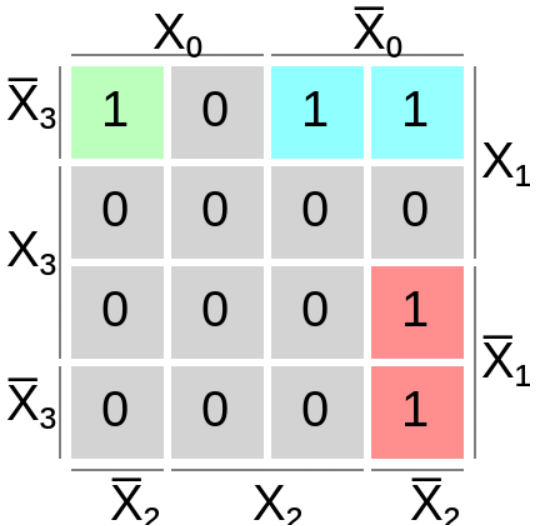
\includegraphics[width=1\linewidth]{course-plis/images/lab1/y3}} а) \\
		\end{minipage}
		\hfill
		\begin{minipage}[h]{0.47\linewidth}
			\center{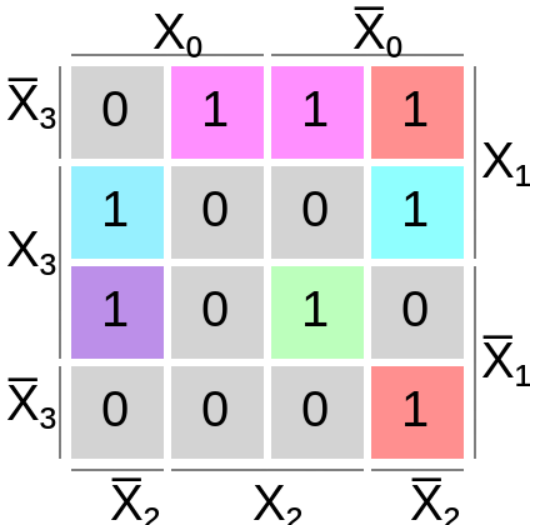
\includegraphics[width=1\linewidth]{course-plis/images/lab1/y2}} \\б)
		\end{minipage}
		\vfill
		\begin{minipage}[h]{0.47\linewidth}
			\center{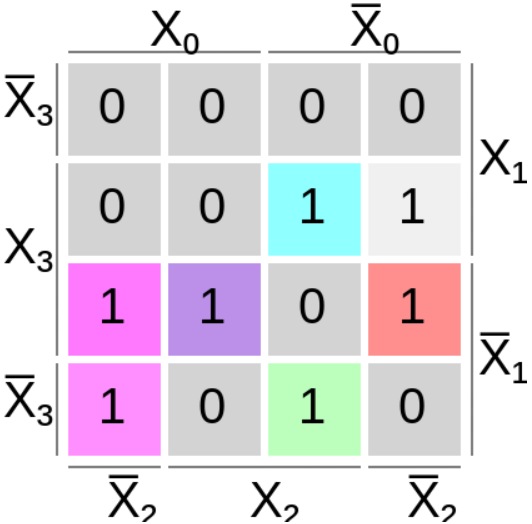
\includegraphics[width=1\linewidth]{course-plis/images/lab1/y1}} в) \\
		\end{minipage}
		\hfill
		\begin{minipage}[h]{0.47\linewidth}
			\center{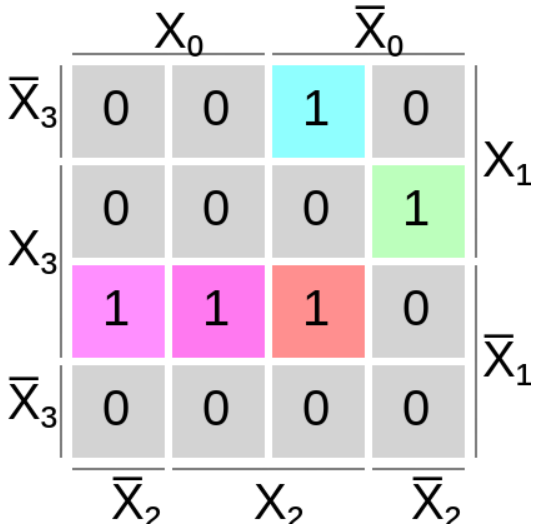
\includegraphics[width=1\linewidth]{course-plis/images/lab1/y0}} г) \\
		\end{minipage}
		\caption{Карты Карно для 4-х переменных для функций а)$Q_3$, б)$Q_2$, в)$Q_2$, г)$Q_1$, д)$Q_0$}
		\label{ris:karno-maps}
	\end{figure}

\section{Минимизация булевых функций}
По построенным картам Карно опишем {МДНФ} для реализации данных функций на вентильном уровне в редакторе Schematic editor САПР Xilinx ISE Design Suite.

\begin{align}
Q_3 &= \bar{X_3}\bar{X_2}\bar{X_1} \vee  X_2 \bar{X_1}\bar{X_0}  \vee \bar{X_3} X_2\bar{X_0} \\
Q_2 &= \bar{X_3} \bar{X_1} \bar{X_0} \vee \bar{X_3} \bar{X_2} X_1 X_0 \vee X_2  \bar{X_1}  X_0 \vee X_2  X_1  \bar{X_0} \vee  X_3  \bar{X_1}  X_0 \\
Q_1 &=  \bar{X_3}\bar{X_1}X_0    \vee  \bar{X_3} \bar{X_2} X_1 \bar{X_0} \vee     \bar{X_3} X_2  X_0  \vee  X_3 \bar{X_2} \bar{X_1}   \vee  X_3 \bar{X_2} X_0 \\
Q_0 &= \bar{X_2} X_1 X_0 \vee \bar{X_3} X_2 \bar{X_1} X_0 \vee \bar{X_3} X_2 X_1 \bar{X_0} \vee X_3 \bar{X_2} X_0
\end{align}

Также опишем \textbf{МКНФ} для реализации булевых функций средствами VHDL в САПР Xilinx ISE Design Suite.
\begin{align}
Q_3 &=\left(
\bar{X_3}\vee \bar{X_1}
\right) 
\cdot 
\left(
X_2\vee \bar{X_1}
\right) 
\cdot  
\left(
\bar{X_2}\vee \bar{X_0}
\right) \\
Q_2 &= \left(
X_2 \vee X_2 \vee X_1 \vee \bar{X_0}
\right) 
\cdot 
\left( 
\bar{X_3} \vee X_2 \bar{X_1}
\right) 
\cdot 
\left(
X_2 \vee  \bar{X_1} \vee X_0
\right)
\cdot \\
& \left(
\bar{X_2}  \vee \bar{X_1} \vee \bar{X_0}
\right)
\cdot 
\left(\bar{X_3} \vee X_1 \vee X_0
\right)\\
Q_1 & = \left( X_3 \vee X_1 \vee X_0 \right) \cdot
\left( \bar{X_3} \vee \bar{X_1 X_0} \right) \cdot
\left( \bar{X_3} \vee \bar{X_2} \right) \cdot \\
& \left(X_3 \vee X_2 \vee \bar{X_1} \vee \bar{X_0}\right) \cdot
\left(\bar{X_2} \vee X_0\right)\\
Q_0 & = \left( X_3 \vee X_2 \vee X_1 \right) \cdot
\left(  X_2 \vee X_0 \right) \cdot
\left( X_1 \vee X_0  \right) \cdot
\left( \bar{X_3} \vee \bar{X_2} \right) \cdot
\left( \bar{X_2} \vee \bar{X_1} \vee \bar{X_0} \right)
\end{align}


\section{Реализация функций в схемотехническом редакторе}
Опишем функции $Q_3$,  $Q_2$, $Q_1$,  $Q_0$ на вентильном уровне в схемотехническом редакторе Schematic editor САПР Xilinx ISE Design Suite (см. Рисунок~\ref{fig:circ-editor}).

\begin{figure}[h!]
	%\hfill
	\begin{minipage}[h]{0.47\linewidth}
		\center{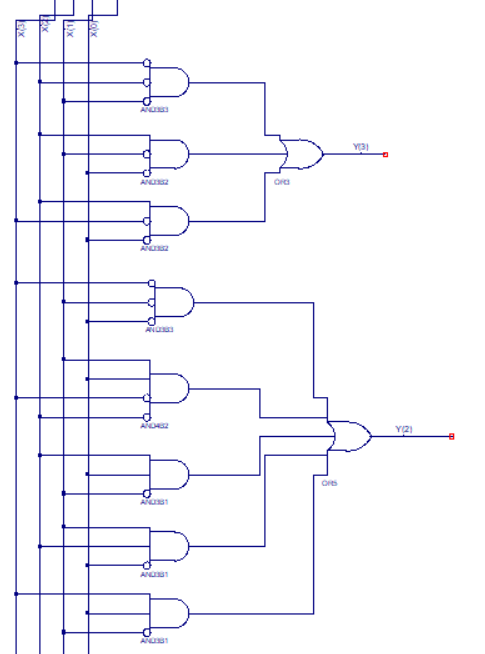
\includegraphics[width=\linewidth]{course-plis/images/lab1/sheme1}} а) \\
	\end{minipage}
	\hfill
	\begin{minipage}[h]{0.47\linewidth}
		\center{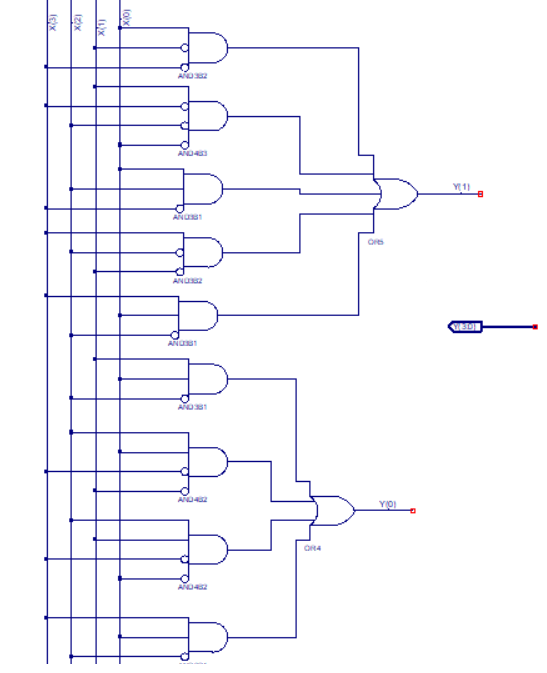
\includegraphics[width=\linewidth]{course-plis/images/lab1/sheme2}} б) \\
	\end{minipage}
	\caption{Схемотехнический редактор а) Лист 1, б) Лист 2}
	\label{fig:circ-editor}
\end{figure}


\newpage
\section{Реализация функций на вентильном уровне}
На основании МКНФ опишем функции $Q_3$,  $Q_2$, $Q_1$,  $Q_0$ на вентильном уровне c помощью языка Verilog.

Исходный код данного модуля приведен в Приложении~\ref{cha:appendix1} на Листинге~\ref{lst:1mknf}.

%\lstinputlisting{/home/denilai/Documents/repos/latex/scripts/mknf.v}

%\newpage
\section{Реализация функций на поведенческом уровне}
На основании построенной ранее Таблицы истинности~\ref{tab:func-table} опишем функции $Q_3$,  $Q_2$, $Q_1$,  $Q_0$ на поведенческом уровне c помощью языка Verilog.

Исходный код данного модуля приведен в Приложении~\ref{cha:appendix1} на Листинге~\ref{lst:1beh}.
%\lstinputlisting{/home/denilai/Documents/repos/latex/scripts/behaviour.v}

%\newpage
\section{Создание проекта САПР Xilinx ISE}

Опишем файл верхнего уровня проекта САПР Xilinx ISE Design Suite, в котором подключим все остальные модули, укажем входные и выходные сигналы. 
Исходный код данного модуля приведен в Приложении~\ref{cha:appendix1} на Листинге~\ref{lst:1top}.
%\lstinputlisting{/home/denilai/Documents/repos/latex/scripts/top.v}


\section{Тестирование и отладка средствами симулятора iSim}
После компоновки проекта, подключения модуля верхнего уровня, проведем верификацию спроектированных моделей с помощью симулятора iSim из состава САПР Xilinx ISE Design Suite. Результаты тестирования можно видеть в Приложении~\ref{cha:appendix2} на Рисунке~\ref{fig:1isim}.

%% TODO: \usepackage{graphicx} required
%\begin{figure}[htpb]
%	\centering
%	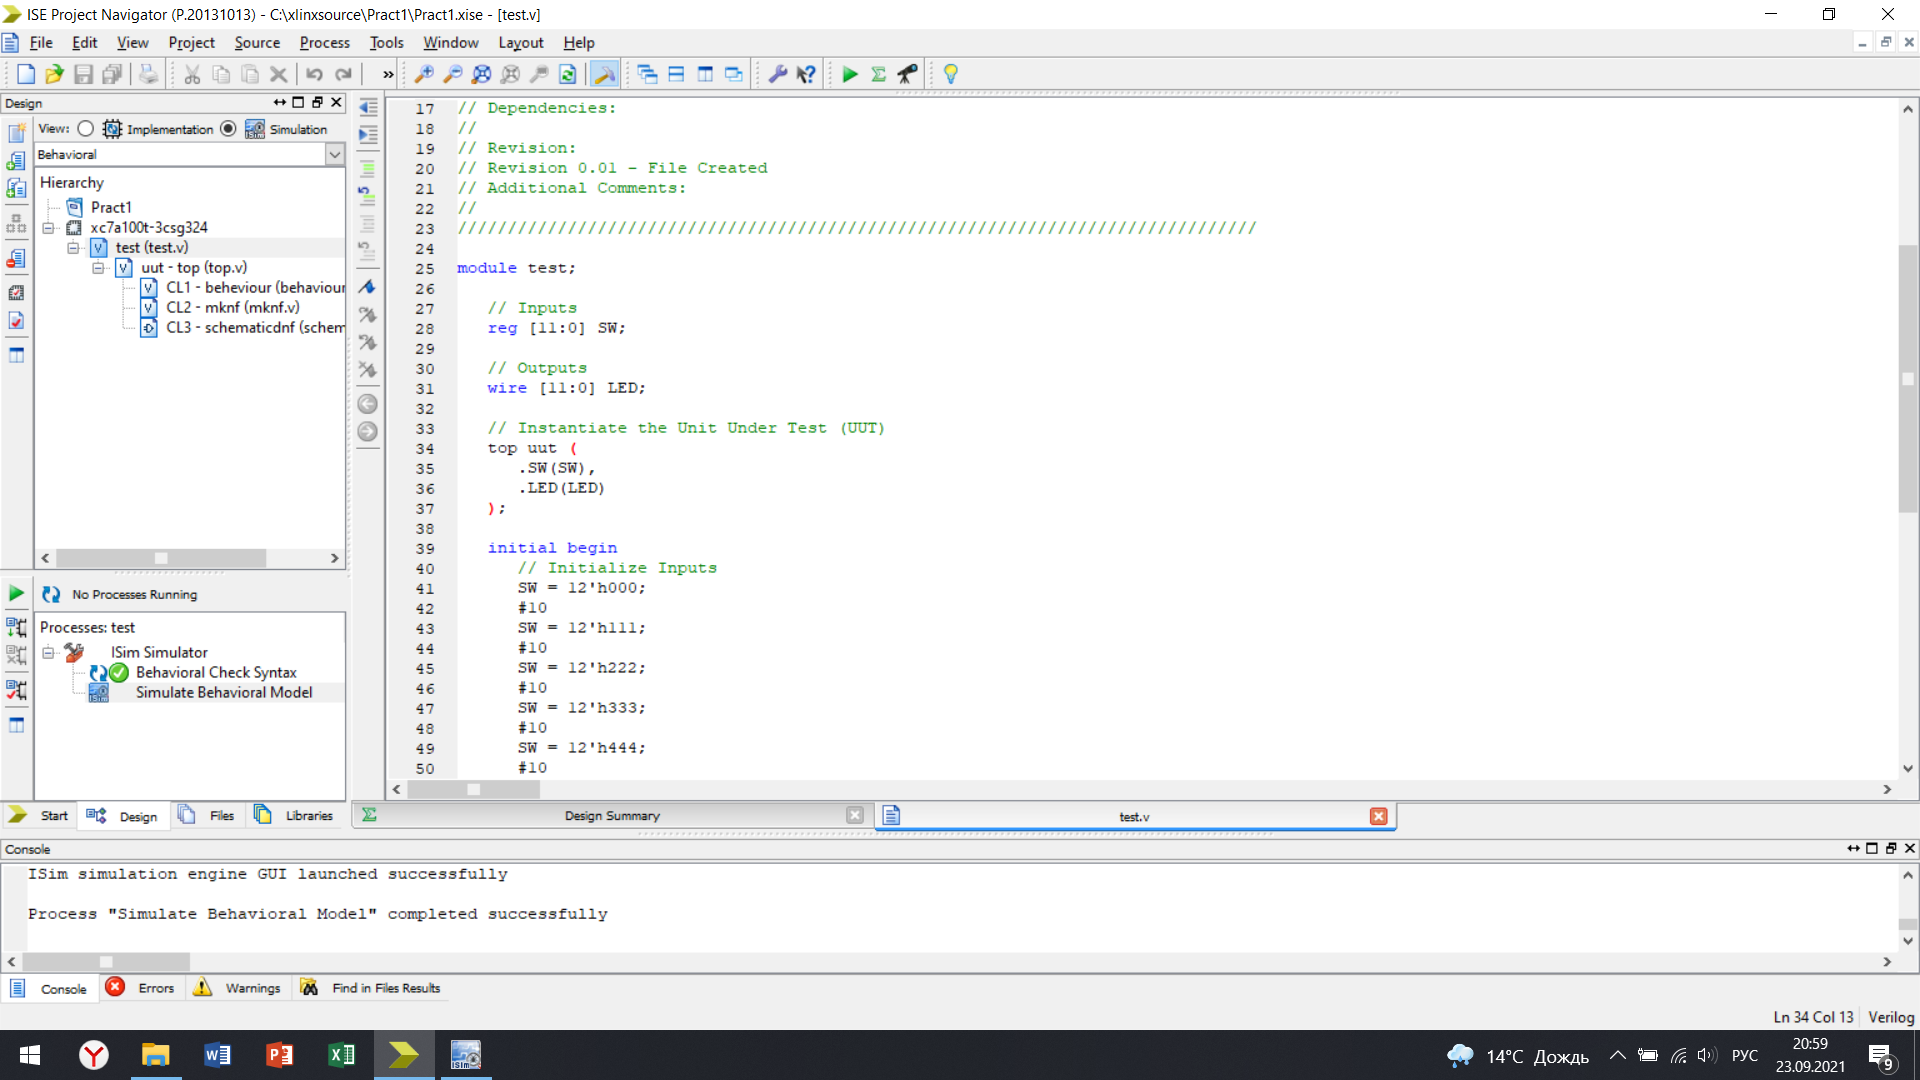
\includegraphics[width=\linewidth]{course-plis/images/lab1/test-result}
%	\caption{Проверка синтаксиса}
%	\label{fig:test-result}
%\end{figure}
%% TODO: \usepackage{graphicx} required
%\begin{figure}[htpb]
%	\centering
%	\includegraphics[width=\linewidth]{course-plis/images/lab1/isim}
%	\caption{Вывод iSim }
%	\label{fig:isim}
%\end{figure}

%\newpage
\section{Вывод}
В данном разделе нами были получены общие навыки работы с программным обеспечением Xilinx ISE Design Suite, изучены основы языка Verilog. С помощью полученных знаний была спроектированы синтезируемые модели комбинационной схемы 4х4, описанной тремя различными способами.

%
%\cite{1},
%\cite{2},
%\cite{3},
%\cite{4},
%\cite{5},
%\cite{6},
%\cite{7},
%\cite{8},
%\cite{9},\\
%\cite{10}\\

\clearpage
\chapter{ПОСТРОЕНИЕ ГЕНЕРАТОРА ПОСЛЕДОВАТЕЛЬНОСТИ}
\label{cha:lab2}
	
\section {Постановка задачи}
Требуется описать конечный автомат, представляющий собой генератор
фиксированной последовательности логических сигналов, в виде синтезируемой модели
на языке Verilog HDL.
Автомат должен иметь интерфейс, представленный на Рисунке~\ref{fig:fsmexample}.

% TODO: \usepackage{graphicx} required
\begin{figure}[h!]
	\centering
	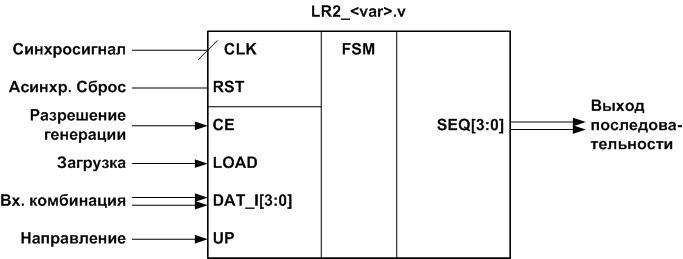
\includegraphics[width=0.6\linewidth]{course-plis/images/lab2/fsm_example}
	\caption{Интерфейс цифрового автомата}
	\label{fig:fsmexample}
\end{figure}


Автомат является синхронным цифровым узлом, срабатывающим по восходящим
фронтам синхросигнала \textit{CLK}. Исключение составляет асинхронный вход сброса \textit{RST},
принудительно устанавливающий регистр автомата в исходное состояние (определяется
вариантом).
Автомат должен реагировать на входные воздействия согласно Таблице~\ref{tab:fsm state}.


\begin{table}[h!]
	\centering
		\caption{Таблица функционирования автомата}
		\small
	\begin{tabular}{|c|c|c|c|c|c|}
		\hline
		\textbf{RST}  & \textbf{CLK}  & \textbf{LOAD}  & \textbf{CE}  & \textbf{UP}  & \textbf{Действие} \\ \hline \hline
		1 & X  & X  & X  & X  & Асинхронный сброс SEQ <= Func(4'h0) \\ \hline
		0 & posedge & 1 & X  & X  & Загрузка SEQ <= Func(DAT\_I) \\ \hline
		0 & posedge & 0 & 1 & 0 & Обратная генерация SEQ <= Func(i-1) \\ \hline
		0 & posedge & 0 & 1 & 1 & Прямая генерация SEQ <= Func(i+1) \\ \hline
		0 & posedge & 0 &  & X  & Хранение SEQ <= SEQ \\ \hline
	\end{tabular}
	\label{tab:fsm state}
\end{table}


Последовательность генерируемых сигналов определяется функцией~\\\textit{Func(i)}, где \textit{i} --- четырехразрядный двоичный индекс, представляющий собой номер элемента
последовательности. 
Инкремент индекса соответствует прямой генерации последовательности.
Декремент индекса соответствует обратной генерации последовательности.

Последовательность для каждого варианта выполнения работы определяется из
таблицы вариантов следующим образом: индекс \textit{i} задан входными комбинациями от \textit{F} до
0 в верхней строке таблицы, а выходные комбинации \textit{Func(i)}, формируемые на выходах
\textit{SEQ[3:0]}, заданы строкой таблицы, соответствующей выбранному варианту.
Допускается использовать различные варианты кодировки состояний автомата.
Автомат может иметь организацию согласно абстрактным моделям Мили или Мура.

\section {Реализация конечного автомата}
Требуется описать конечный автомат, представляющий собой генератор
фиксированной последовательности логических сигналов, в виде синтезируемой модели
на языке Verilog HDL согласно данной таблице истинности и вектор-функции (см. Таблицу~\ref{tab:func-vector}).

\begin{table}[h!]
	\centering
	\caption{Вектор-функция}
		\begin{tabular}{|c|c|c|c|c|c|c|c|c|c|c|c|c|c|c|c|}
			\hline
			F & E & D & C & B & A & 9 & 8 & 7 & 6 & 5 & 4 & 3 & 2 & 1 & 0 \\ \hline\hline
			0 & 4 & 4 & 8 & 3 & 0 & 7 & 2 & 2 & D & 7 & C & 5 & 2 & A & C \\ \hline
		\end{tabular}
		\label{tab:func-vector}
\end{table}

\section{Структурная схема автомата}
Построим структурную схему цифрового устройства. Используем делитель частоты для снижения частоты тактового генератора, фильтр дребезга для использования кнопок в качестве устройств ввода (см. Рисунок~\ref{fig:fsm-struct}).
% TODO: \usepackage{graphicx} required
\begin{figure}[htpb]
	\centering
	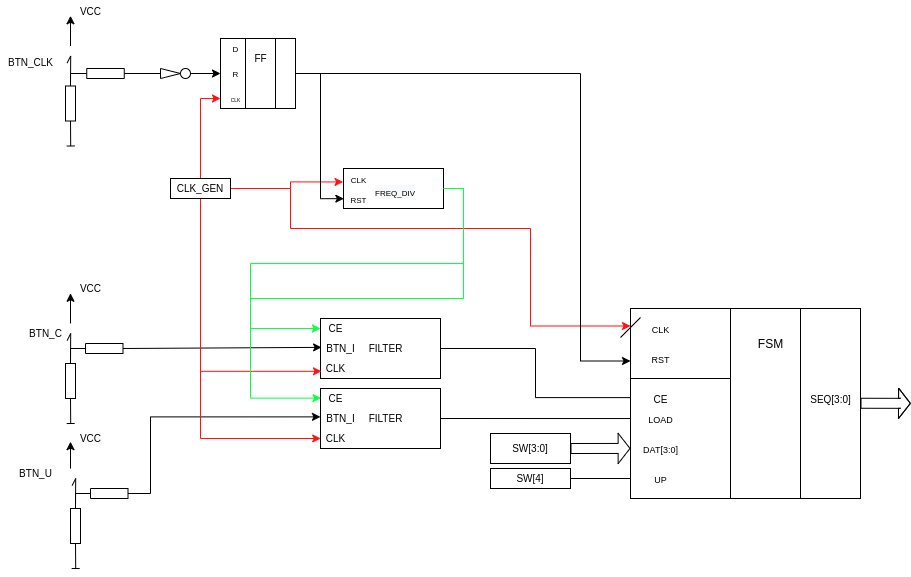
\includegraphics[width=\linewidth]{course-plis/images/lab2/fsm-struct}
	\caption{Структурная схема  устройства}
	\label{fig:fsm-struct}
\end{figure}


\section{Кодировка состояний автомата в двоичной и шестнадцатиричной системах}
Опишем модуль behaviour.v, указав в нем состояния автомата, приведенные в шестнадцатеричной системе.
Исходный код данного модуля приведен в Приложении~\ref{cha:appendix1} на Листинге~\ref{lst:1beh}.


%\newpage
\section{Граф состояний}
Опишем граф перехода цифрового автомата согласно указанным режимам работы (переход в следующее или предыдущее состояние, загрузка состояния, хранение, сброс) (см. Рисунок~\ref{fig:graph}).
% TODO: \usepackage{graphicx} required
\begin{figure}[h!]
	\centering
	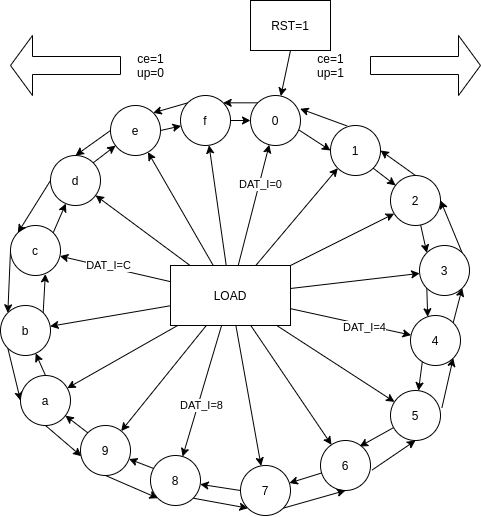
\includegraphics[width=0.4\linewidth]{course-plis/images/lab2/graph}
	\caption{Граф переходов}
	\label{fig:graph}
\end{figure}

\newpage
\section{Создание проекта САПР Xilinx ISE}

\paragraph{Автомат генератор последовательности.}
Реализуем на языке Verilog модуль, описывающий цифровой автомат. 
Исходный код данного модуля приведен в Приложении~\ref{cha:appendix1} на Листинге~\ref{lst:2fsm}.
\paragraph{Делитель частоты.}
Реализуем на языке Verilog модуль, описывающий делитель частоты.
Исходный код данного модуля приведен в Приложении~\ref{cha:appendix1} на Листинге~\ref{lst:2freq-div}.

\paragraph{Фильтр дребезга кнопок.}
Реализуем на языке Verilog модуль, описывающий фильтр дребезга.
Исходный код данного модуля приведен в Приложении~\ref{cha:appendix1} на Листинге~\ref{lst:2filter}.

\paragraph{Модуль верхнего уровня.}
Реализуем на языке Verilog модуль верхнего уровня.
Исходный код данного модуля приведен в Приложении~\ref{cha:appendix1} на Листинге~\ref{lst:2top}.


\paragraph{Тестовое окружение.}
Реализуем на языке Verilog модуль, описывающий тестовое окружение, описывающее входные воздействия для данной модели.
Исходный код данного модуля приведен в Приложении~\ref{cha:appendix1} на Листинге~\ref{lst:2fsm-test}.


\section{Тестирование и отладка средствами симулятора iSim}
После компоновки проекта, подключения модуля верхнего уровня, проведем верификацию спроектированных моделей с помощью симулятора iSim из состава САПР Xilinx ISE Design Suite. Результаты тестирования можно видеть в Приложении~\ref{cha:appendix2} на Рисунках~\ref{fig:2isim1}.~\ref{fig:2isim2}.



\section{Вывод}
  В данном разделе нами были получены общие навыки работы с программным обеспечением Xilinx ISE Design Suite, изучены основы языка Verilog.

С помощью полученных знаний был спроектирован конечный автомат, представляющий собой генератор
фиксированной последовательности логических сигналов, в виде синтезируемой модели.


\clearpage
\chapter{РАЗРАБОТКА АНАЛИЗАТОРА ПОСЛЕДОВАТЕЛЬНОСТИ}
\section{Постановка задачи}	



Требуется разработать цифровой узел на основе отладочной платы Digilent Nexys 4,
представляющий собой анализатор фиксированной последовательности логических
сигналов. Узел должен обеспечивать индикацию ожидаемых и вводимых элементов
последовательности посредством входящих в состав отладочной платы семисегментных
индикаторов согласно данному заданию.

Узел должен быть реализован в виде синтезируемой модели на языке Verilog HDL.

Автомат должен иметь интерфейс, представленный на Рисунке~\ref{fig:interface-pract3}.

% TODO: \usepackage{graphicx} required
\begin{figure}[h!]
	\centering
	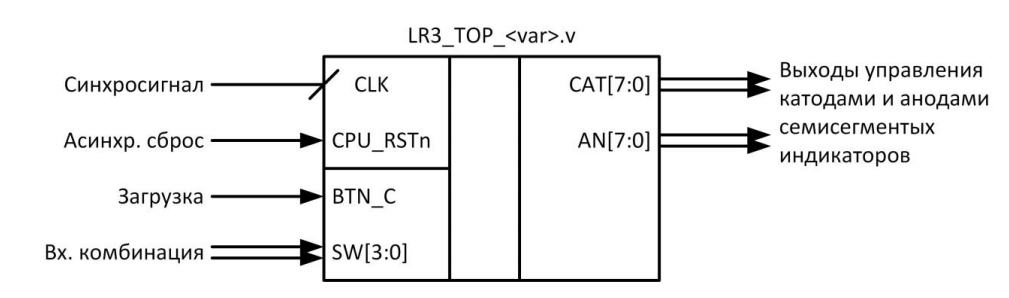
\includegraphics[width=0.7\linewidth]{course-plis/images/lab3/interface-pract3}
	\caption{Интерфейс модели цифрового узла}
	\label{fig:interface-pract3}
\end{figure}


Разрабатываемое устройство является синхронным цифровым узлом,
срабатывающим по восходящим фронтам синхросигнала CLK. Исключение составляет
асинхронный вход сброса CPU\_RSTn, принудительно устанавливающий все регистры
узла в исходное состояние. Подача сигнала сброса на вход узла осуществляется
посредством соответствующей кнопки (CPU\_RSTn) отладочной платы.

Распознавание элементов последовательности осуществляется четверками, т.е.
необходимо обеспечить последовательную загрузку в узел элементов Y c номерами 0-3, 4-
7, 8-B, C-F для успешного распознавания последовательности. При осуществлении ввода
значения, не соответствующего текущему ожидаемому элементу последовательности,
необходимо повторить ввод всей четверки элементов заново.




Индикация работы узла посредством двух блоков семисегментных индикаторов подчиняется следующим правилам:
\begin{enumerate}
	\item Левый блок семисегментных индикаторов отображает ожидаемый (младший
	разряд) и введенные (три старших разряда) элементы последовательности в объеме
	распознаваемой четверки.
	\item  Правый блок семисегментных индикаторов отображает предысторию ввода
	комбинаций последовательности. Последняя введенная комбинация отображается в
	младшем разряде блока.
	\item  Не задействованные в текущий момент времени семисегментные индикаторы на
	обоих блоках должны находится в выключенном состоянии.
	\item Обновление отображаемых значений на обоих блоках семисегментных
	индикаторов рекомендуется выполнять с частотой от 60Гц до 200Гц.
\end{enumerate}


\section{Моделирование цифрового устройства}

В ходе выполнения данного задания было реализовано синхронное устройство. Его работы была организована по восходящему фронту синхросигнала, асинхронный сброс --- по нисходящему фронту сигнала CPU\_RSTn. 

Приведем таблицу состояний устройства (см. Таблицу~\ref{tab:states}). Текущее состояние цифрового устройства зависит от последнего введенного пользователем с помощью движковых переключателей элемента последовательности. 

\begin{table}[h!]
	\centering
	\small
	\caption{Состояния цифрового устройства}
	\begin{tabular}{|c|c|c|c|c|c|c|c|c|c|c|c|c|c|c|c|c|c|}
		\hline
		Состояние & 16& 15&	14	&13	&12&11&	10&	9&	8&	7&	6&	5&	4&	3&	2&	1&	0\\ \hline\hline
		Значение & 0 & 4 & 4 & 8 & 3 & 0 & 7 & 2 & 2 & D & 7 & C & 5 & 2 & A & C&-- \\ \hline\hline
		Разряд & F & E & D & C & B & A & 9 & 8 & 7 & 6 & 5 & 4 & 3 & 2 & 1 & 0 &--\\ \hline
	\end{tabular}
	
	\label{tab:states}
\end{table}

Перечислим функциональные узлы, которые уже были реализованы ранее. 

\begin{enumerate}
	\item Делитель частоты. Реализован в разделе~\ref{cha:lab2}.
	\item Фильтр дребезга кнопок. Реализован в разделе~\ref{cha:lab2}.
	\item Конечный автомат генератор последовательности. Реализован в разделе~\ref{cha:lab2}.
\end{enumerate}

Приведем построенный граф состояний цифрового устройства (см. Рисунок~\ref{fig:state-graph-pract3}). Переход в следующее состояние происходит только в случае ввода верного элемента последовательности. При неправильном вводе цифровое устройство переходит в ближайшее пройденное состояние, номер которого кратен 4. Номер состояния, в которое перейдет устройство в случае некорректного ввода можно вычислить по формуле $S_{i+1}=(S_i \div 4) \cdot 4$.

% TODO: \usepackage{graphicx} required
\begin{figure}[h!]
	\centering
	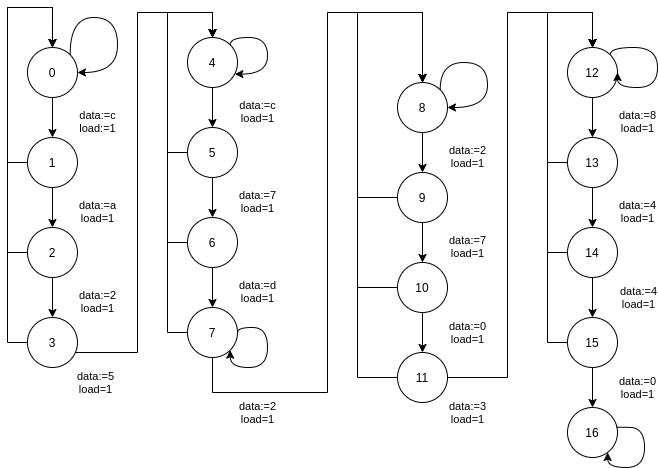
\includegraphics[width=0.7\linewidth]{course-plis/images/lab3/state-graph-pract3}
	\caption{Граф состояний}
	\label{fig:state-graph-pract3}
\end{figure}

%\newpage
Приведем блок схему работы устройства (см. Рисунок~\ref{fig:algorithm-pract3}). Значение Х представляет
собой номер элемента цифровой последовательности, ввод значения которого (Y)
ожидается. Значения Y каждого элемента цифровой последовательности определяются
вариантом задания.

% TODO: \usepackage{graphicx} required
\begin{figure}[h!]
	\centering
	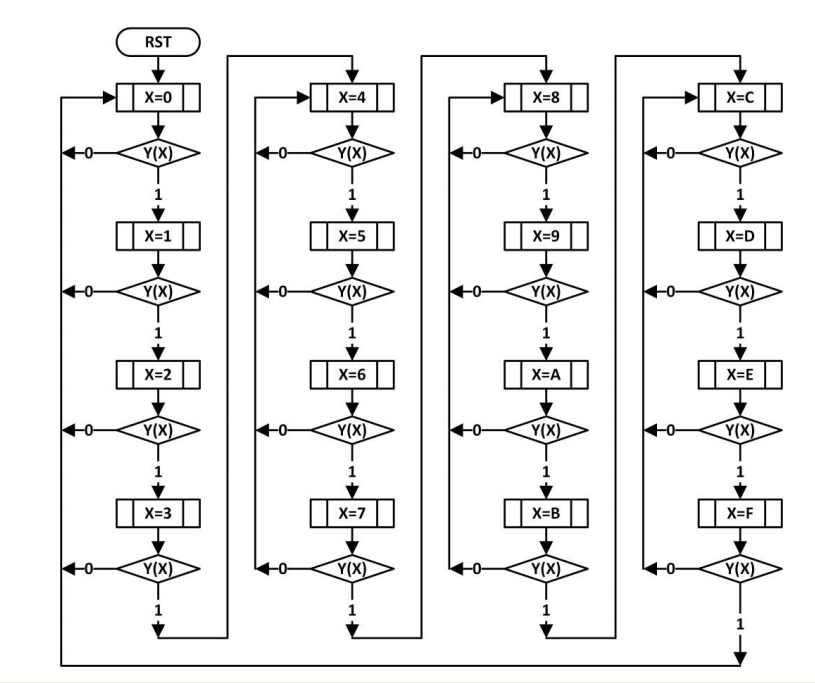
\includegraphics[width=0.68\linewidth]{course-plis/images/lab3/algorithm-pract3}
	\caption{Алгоритм распознавания последовательности}
	\label{fig:algorithm-pract3}
\end{figure}

Приведем структурную схему синхронного цифрового узла (см. Рисунок~\ref{fig:unit-pract3}).

% TODO: \usepackage{graphicx} required
\begin{figure}[h!]
	\centering
	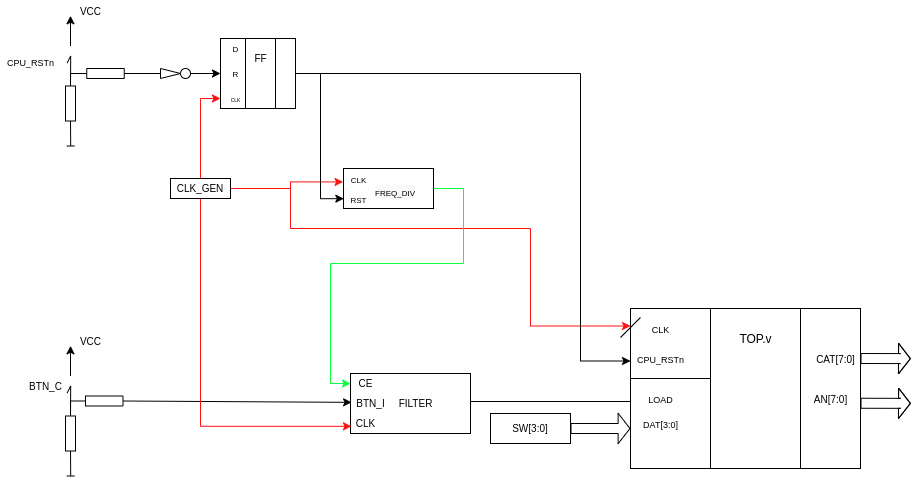
\includegraphics[width=0.8\linewidth]{course-plis/images/lab3/unit-pract3}
	\caption{Структурная схема узла}
	\label{fig:unit-pract3}
\end{figure}


\section{Описание принципа работы}

Главный алгоритм работы цифрового устройства --- контроль ввода шестнадцатеричных чисел с возможностью повторного задания последовательности.

Данный алгоритм описан в файле {seqAuto.v}. Его содержание приведено в приложении~\ref{cha:appendix1} на Листинге~\ref{lst:3seq-auto}.

Сначала производится инициализация переменных, затем, если есть необходимость обновить изображение на дисплее (переменная \texttt{updateDisplay}), анализируется текущее состояние дисплея и пользовательский ввод. 

Если номер состояния автомата кратен четырем, то отображается только левый разряд на левом дисплее. На это место выводится соответствующее значение функции, а в остальных 3 разряда левого дисплея отображаются нули.

Если номер состояния автомата не кратен четырем, то следует перезаписать все разряды на левом дисплее на один разряд влево, записать в освободившийся разряд записываем очередное значение вектор--функции. 

В конце переменная \texttt{updateDisplay} устанавливается в нуль. 

Если пользователь подал сигнал на загрузку числа, производятся следующие действия:

Все разряды на правом дисплее перезаписываются на один разряд влево, в освободившийся разряд записывается заданное пользователем число. 

Если пользователь произвел верный ввод, автомат переводится в следующее состояние. В случае ввода неправильного переводим автомат в ближайшее пройденное состояние, номер которого кратен четырем.

В конце переменная \texttt{updateDisplay} устанавливается в единицу. 

\section{Создание проекта САПР Xilinx ISE}

\paragraph{Автомат анализатор входной последовательности.}
Был описан файл seqAuto.v, реализующий главный алгоритм управления цифровым устройством, который был описан в предыдущей секции (см. Приложение~\ref{cha:appendix1} Листинг~\ref{lst:3seq-auto}).


\paragraph{Фильтр дребезга кнопок.}
Был использован ранее созданный модуль, реализующий фильтр дребезга кнопок.
Исходный код данного модуля приведен в Приложении~\ref{cha:appendix1} на Листинге~\ref{lst:2filter}.

\paragraph{Делитель частоты.}
Был использован ранее созданный модуль, реализующий делитель частоты, применяемый в данном проекте для снижения выходных характеристик частотного генератора для подбора оптимального режима работы с семисегментными индикаторами.
Исходный код данного модуля приведен в Приложении~\ref{cha:appendix1} на Листинге~\ref{lst:2freq-div}.


\paragraph{Драйвер для работы с семисегментыми индикаторами.}
Был реализован модуль NexysDisplay.v на языке Verilog, описывающий работу с семисегментыми индикаторами. В его составе используется дешифратор, которых активирует сегменты индикатора в зависимости от текущего обрабатываемого шестнадцатеричного числа.

 Исходный код данного модуля приведен в Приложении~\ref{cha:appendix1} на Листинге~\ref{lst:3display}.

\paragraph{Пользовательская функция.}
Приведем содержание файла outFunc.v, описывающего представление бинарной вектор--функции, значения которой сравниваются с пользовательским вводом. 
Исходный код данного модуля приведен в Приложении~\ref{cha:appendix1} на Листинге~\ref{lst:1beh}.

\paragraph{Сигнальный дешифратор.}
Приведем содержание файла SevenSegDec.v, описывающего работу сигнального дешифратора для работы с семисегментыми индикаторами.
Исходный код данного модуля приведен в Приложении~\ref{cha:appendix1} на Листинге~\ref{lst:3decode}.

\paragraph{Модуль верхнего уровня.}
Приведем содержание файла top.v, описывающего работу модуля верхнего уровня, объединяющего все файлы и организующего работу с устройством.
Исходный код данного модуля приведен в Приложении~\ref{cha:appendix1} на Листинге~\ref{lst:3top}.


\section{Тестирование и отладка средствами симулятора ISim}

После реализации функциональных узлов устройства было проведено тестирование работы спроектированного цифрового устройства средствами САПР Xilinx ISE 14. 

Результаты тестирования приведены в Приложении~\ref{cha:appendix2} на Рисунках~\ref{fig:3page-1}-\ref{fig:3page-6}.



\section{Вывод}
В данном разделе нами были получены общие навыки работы с программным обеспечением Xilinx ISE Design Suite, изучены основы языка Verilog.

С помощью полученных знаний был спроектирован и разработан цифровой узел на основе отладочной платы Digilent Nexys 4, представляющий собой анализатор фиксированной последовательности логических
сигналов. 



\clearpage
\chapter{МОДЕЛИРОВАНИЕ ФУНКЦИОНАЛЬНОГО УЗЛА УПРАВЛЕНИЯ МАТРИЧНЫМ ДИСПЛЕЕМ}
\label{cha:lab4}
\section{Постановка задачи}	

Требуется разработать модель цифрового логического устройства объёме ПЛИС Spartan-3E XC3S500E4PQ208C, сочетающую в себе
функциональные узлы делителя частоты 1кГц, фильтра дребезга контактов
кнопки и конечного автомата генератора последовательности.

Цифровой узел должен выводить на матричный дисплей размером восемь строк на восемь столбцов шестнадцатеричную цифру, значение которой определяется данной таблицы истинности и вектор-функции (Таблица~\ref{tab:4func-vector}).




\begin{table}[h!]
	\centering
	\caption{Вектор-функция}
	\begin{tabular}{|c|c|c|c|c|c|c|c|c|c|c|c|c|c|c|c|}
		\hline
		F & E & D & C & B & A & 9 & 8 & 7 & 6 & 5 & 4 & 3 & 2 & 1 & 0 \\ \hline\hline
		0 & 4 & 4 & 8 & 3 & 0 & 7 & 2 & 2 & D & 7 & C & 5 & 2 & A & C \\ \hline
	\end{tabular}
	\label{tab:4func-vector}
\end{table}


Организовать на языке Verilog тестовый модуль, осуществляющий верификацию написанных модулей. Тестовое окружение должно моделировать работу устройства на частоте 1 МГц. Функциональные узлы делителя частоты и фильтра в тестировании могут не участвовать.



\section{Моделирование цифрового устройства}
Приступим к реализации модели цифрового узла. Приведем структурную схему синтезируемой части проекта (см. Рисунок~\ref{fig:struct-scheme}).


\begin{figure}[h!]
	\centering
	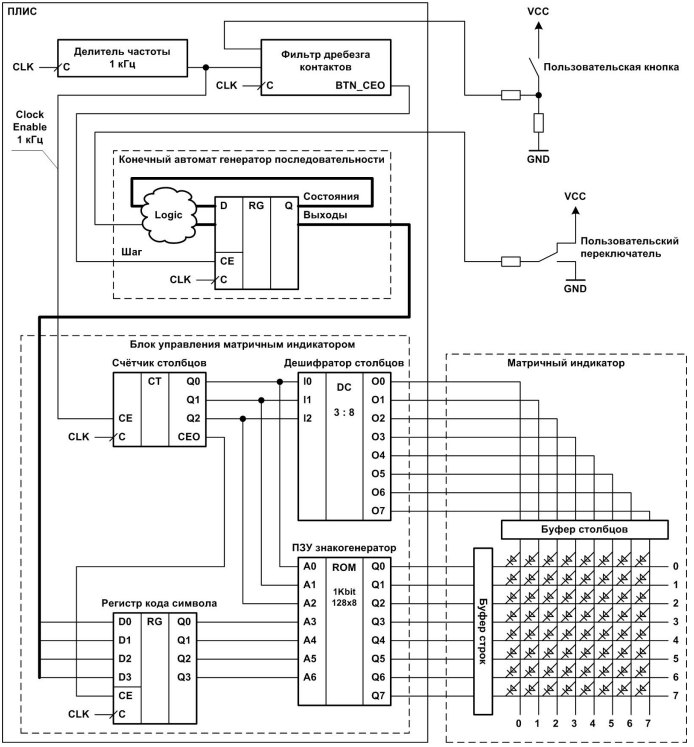
\includegraphics[width=0.6\linewidth]{course-plis/images/lab4/struct-scheme}
	\caption{Структурная схема синтезируемой части проекта}
	\label{fig:struct-scheme}
\end{figure}


Перечислим функциональные узлы, которые уже были реализованы ранее. 

\begin{enumerate}
	\item Делитель частоты. Реализован в разделе~\ref{cha:lab2}.
	\item Фильтр дребезга кнопок. Реализован в разделе~\ref{cha:lab2}.
	\item Конечный автомат генератор последовательности. Реализован в разделе~\ref{cha:lab2}.
\end{enumerate}

Процесс создания данных модулей не будет освещаться в настоящем разделе. 

\section{Принцип работы матричного индикатора}
Рассмотрим принцип работы матричного индикатора.
Вывод организуем по столбцам. В определённый момент времени активным является столбец,
и любые из восьми светодиодов активного столбца могут подсвечиваться
одновременно. 

Это даёт возможность увидеть одноцветное изображение,
выводимое на матричный дисплей, непосредственно на временной
диаграмме. Принцип вывода информации на матричный индикатор на
примере символа «9» показан на Рисунке~\ref{fig:display-principe}.

\begin{figure}[h!]
	\centering
	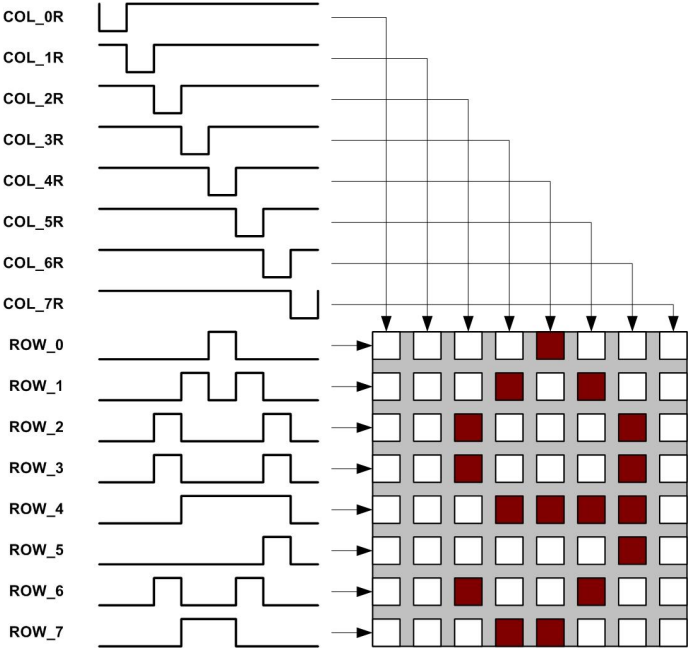
\includegraphics[width=0.5\linewidth]{course-plis/images/lab4/display-principe}
	\caption{Вывод символа на матричный индикатор}
	\label{fig:display-principe}
\end{figure}


\section{Создание проекта САПР Xilinx ISE}

\paragraph{Блок управления матричным индикатором}.
Была реализована модель функционального узла, выполняющего роль блока управления матричным дисплеем размеров восемь строк на восемь столбцов. Его работа организована по восходящему фронту синхросигнала CLK, сброс --- по восходящему фронту сигнала RST. 

Устройство содержит в себе счетчик столбцов, дешифратор столбцов, выбирающий в определенный момент времени только один активный столбец, а также элемент памяти (ПЗУ) хранящий шаблоны всех шестнадцатеричных чисел. ПЗУ будет использоваться знакогенератором для формирования символа из четырехразрядного двоичного входа, поданного в качестве входного сигнала.

Число шаблонов определяется числом символов и равно 16.
Объём ПЗУ знакогенератора составляет 1 кбит или 128 байт.

Младшие три разряда адреса ПЗУ выбирают текущий столбец в рамках
одного шаблона.
Старшие четыре разряда адреса ПЗУ выбирают текущий шаблон.

Шаблоны шестнадцатеричных чисел будут сформированы вручную и занесены в файл. В ходе моделирования работы устройства ПЗУ блока управления индикатором будет проинициализировано значениями, указанными в файле.

Исходный код данного функционального блока приведен в Приложении~\ref{cha:appendix1} в Листинге~\ref{lst:4lcd}.


\paragraph{Модуль верхнего уровня.}
Был описан модуль верхнего уровня, в которым подключены функциональные узлы моделируемого цифрового устройства согласно схеме, приведенной на Рисунке~\ref{fig:struct-scheme}.

В данном модуле использован делитель частоты DIV\_1MHz, преобразующий сигнал частотой 48МГц в сигнал частотой 1МГц.

Генератор последовательности fsm подключен к драйверу матричного дисплея lcd. Так текущее состояние автомата будет отображаться на матричном индикаторе.

Исходный код данного модуля приведен в Приложении~\ref{cha:appendix1} в Листинге~\ref{lst:4top}.

\paragraph{Тестовый модуль.}
Также был реализован модуль, который определяет тестовое окружение рассматриваемой части цифрового логического устройства. 

В модуле верхнего уровня описан генератор тактового сигнала частотой 48 МГц, использованный в качестве тактового сигнала для всех синхронных функциональных узлов в составе устройства. 

Сигнал с частотой 1МГц используется как сигнал разрешения счета для конечного автомата генератора последовательности, блока управления матричным индикатором, фильтра дребезга кнопок. 

Исходный код данного модуля приведен в Приложении~\ref{cha:appendix1} в Листинге~\ref{lst:4test-top}.


\section{Тестирование и отладка средствами симулятора iSim}
После компоновки проекта, подключения модуля верхнего уровня, была произведена верификация спроектированных моделей с помощью симулятора iSim из состава САПР Xilinx ISE Design Suite. Результаты тестирования можно видеть в Приложении~\ref{cha:appendix2} на Рисунках~\ref{fig:4isim}, на котором различимы повернутые на 180 градусов шестнадцатеричные числа, соответствующие исходной вектор-функции (см. Рисунок~\ref{tab:4func-vector}).


\section{Вывод}

В данном разделе нами были получены общие навыки работы с программным обеспечением Xilinx ISE Design Suite, изучены основы языка Verilog.

С помощью полученных знаний был спроектирован функциональный узел по управлению матричным индикатором, который был использован для вывода текущего состояния автомата--генератора последовательности.



\clearpage
\chapter{РЕАЛИЗАЦИЯ ГЕНЕРАТОРА ШИМ}
\section{Постановка задачи}	
Требуется разработать модель цифрового логического устройства объёме ПЛИС Spartan-3E XC3S500E4PQ208C, сочетающую в себе
функциональные узлы делителя частоты 1кГц, фильтра дребезга контактов
кнопки и конечного автомата генератора последовательности.

Центральным узлом схемы является 64-разрядный сдвиговый регистр.
Исходное состояние сдвигового регистра определяется заданной в виде вектор-функции таблицей истинности (см. Таблицу~\ref{tab:4func-vector}).


\begin{table}[h!]
	\centering
	\small
	\caption{Вектор-функция}
	\begin{tabular}{|c|c|c|c|c|c|c|c|c|c|c|c|c|c|c|c|}
		\hline
		F & E & D & C & B & A & 9 & 8 & 7 & 6 & 5 & 4 & 3 & 2 & 1 & 0 \\ \hline\hline
		0 & 4 & 4 & 8 & 3 & 0 & 7 & 2 & 2 & D & 7 & C & 5 & 2 & A & C \\ \hline
	\end{tabular}
	\label{tab:5func-vector}
\end{table}

Сдвиговый регистр после снятия сигнала асинхронного сброса RST
должен содержать значения, соответствующие варианту, как показано на
Рисунке~\ref{fig:set-reset}.


\begin{figure}
	\centering
	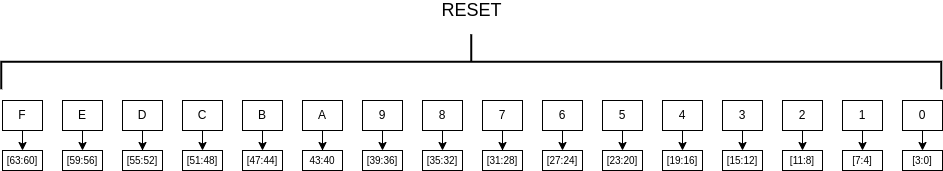
\includegraphics[width=0.75\linewidth]{course-plis/images/lab5/set-reset}
	\caption{Исходное состояние сдвигового регистра}
	\label{fig:set-reset}
\end{figure}



Во время штатного функционирования, при деактивированном сигнале
сброса RST сдвиговый регистр способен выполнять две операции.
Первая операция --- циклический сдвиг влево на 4 разряда, выполняется при
<<1>> на входе SHIFT\_4B\_L, как показано на Рисунке~\ref{fig:leftshift}.

\begin{figure}[h!]
	\centering
	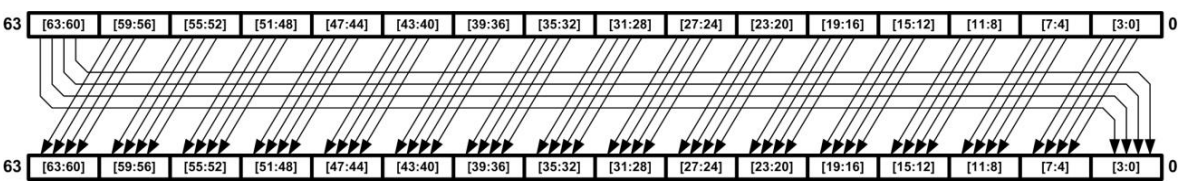
\includegraphics[width=0.8\linewidth]{course-plis/images/lab4/left_shift}
	\caption{Операция сдвига влево}
	\label{fig:leftshift}
\end{figure}

Вторая операция – циклический сдвиг вправо на 4 разряда, выполняется
при <<0>> на входе SHIFT\_4B\_L и <<1>> на входе SHIFT\_4B\_R, как показано на Рисунке~\ref{fig:rightshift}.


\begin{figure}[h!]
	\centering
	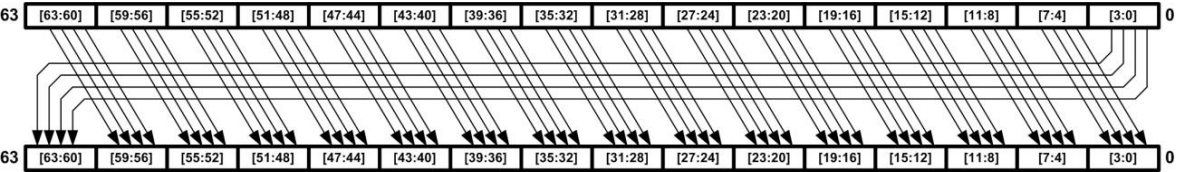
\includegraphics[width=0.8\linewidth]{course-plis/images/lab4/right_shift}
	\caption{Операция сдвига вправо}
	\label{fig:rightshift}
\end{figure}





Сигналы, управляющие сдвиговым регистром, формируются фильтрами
дребезга контактов по нажатию на две пользовательские кнопки.
Выходы сдвигового регистра подаются на два блока индикации.

Первый блок использует светодиоды общего назначения, которые
управляются в режиме регулировки яркости свечения с помощью широтноимпульсного сигнала.

Второй блок индикации использует матричный индикатор, на который
выводятся все 64 разряда сдвигового регистра. Блок управления матричным индикатором коммутирует разряды сдвигового регистра согласно Рисунку~\ref{fig:display-out}.
Такая организация вывода позволяет увидеть изображение, выводимое на
индикатор, непосредственно на временной диаграмме.


\begin{figure}[h!]
	\centering
	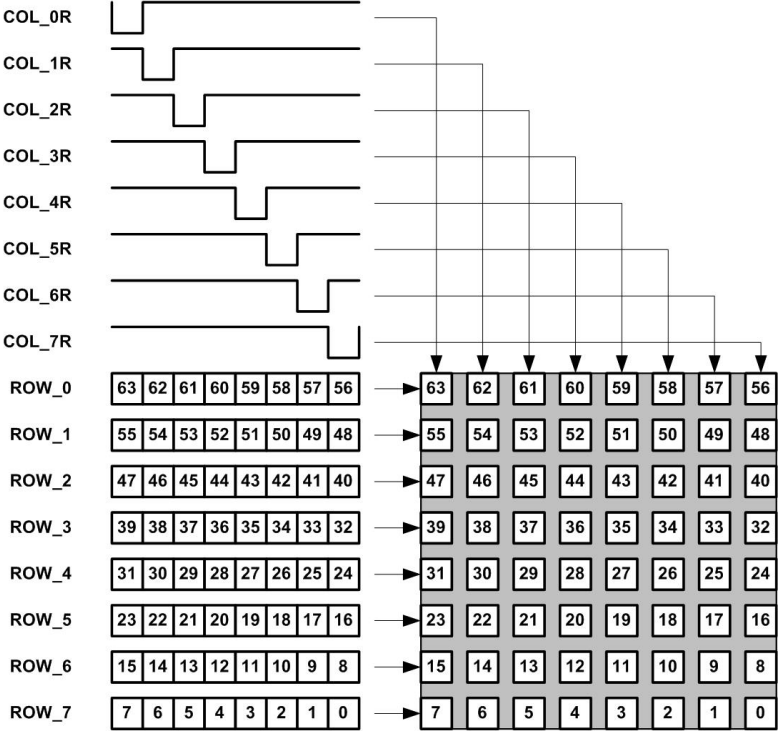
\includegraphics[width=0.45\linewidth]{course-plis/images/lab4/display-out}
	\caption{Вывод содержимого регистра на матричный индикатор}
	\label{fig:display-out}
\end{figure}


В процессе выполнения задания необходимо описать на
языке Verilog модель генератора широтно-импульсного сигнала, имеющий интерфейс, приведенный на Рисунке~\ref{fig:pwm-interface}.

\begin{figure}[h!]
	\centering
	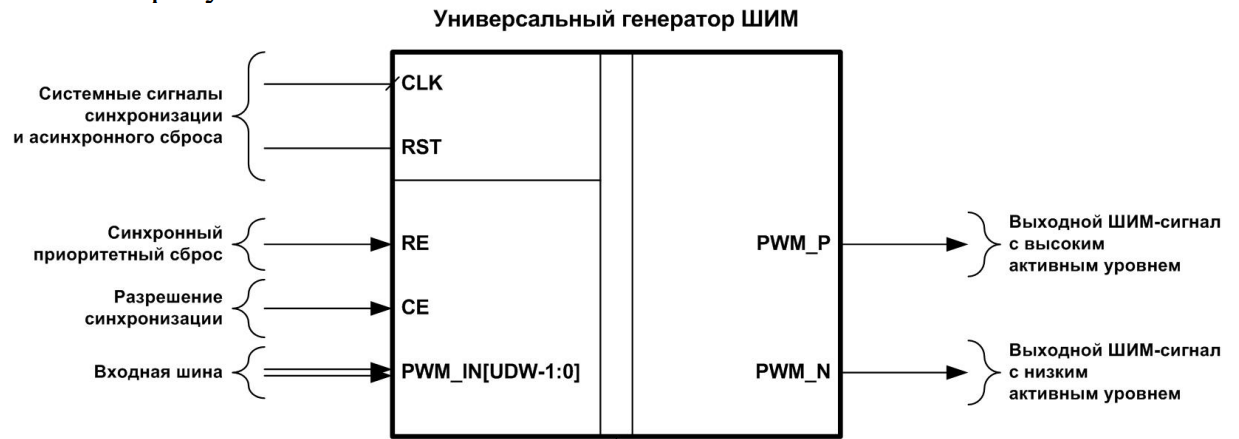
\includegraphics[width=0.55\linewidth]{course-plis/images/lab4/pwm-interface}
	\caption{Интерфейс генератора широтно-импульсного сигнала}
	\label{fig:pwm-interface}
\end{figure}


\section{Принцип широтно-импульсной модуляции}
Принцип широтно-импульсной модуляции (Pulse-Width
Modulation --- \\PWM) заключается в использовании двух уровней сигнала:
низкого и высокого, или <<0>> и <<1>>, соответственно, чередующихся с
фиксированным периодом, но с различной длительностью каждого уровня в
объёме периода.


\section{Реализация генератора ШИМ}


Синтезируемая модель генератора ШИМ-сигналов имеет параметр UDW,
определяющий разрядность входной шины и число состояний управляющего
автомата в объёме периода сигнала (частоту дискретизации). 

Именно этот
параметр обеспечивает универсальность модели.

\begin{figure}[h!]
	\centering
	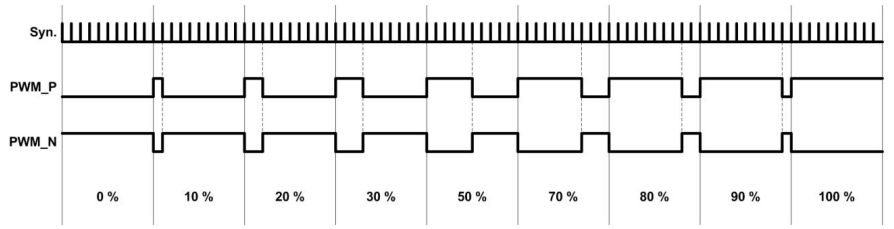
\includegraphics[width=0.6\linewidth]{course-plis/images/lab4/5principe}
	\caption{Принцип широтно-импульсной модуляции}
	\label{fig:5principe}
\end{figure}


%\begin{table}[h!]
%	\centering
%	\small
%	\begin{tabular}{|c|p{0.6\linewidth}|}
%		\hline
%		Параметр & Назначение \\ \hline
%		UDW & Определяет разрядность входной шины и число состояний управляющего
%		автомата в объёме периода сигнала (частоту дискретизации) \\ \hline
%		PWM\_P & Выходной ШИМ-сигнал с высоким активным сигналом \\\hline
%		PWM\_N & Выходной ШИМ-сигнал с низким активным сигналом \\\hline
%	\end{tabular}
%\end{table}
Число возможных входных комбинаций PWM\_IN, задающих коэффициент
заполнения периода активным уровнем сигнала (<<1>> -- для PWM\_P, <<0>> -- для
PWM\_N), составляет $2UDW$ штук. При этом комбинация из всех <<0>> задаёт
коэффициент 0\%, а комбинация из всех <<1>> – коэффициент 100\%. 

Период выходного сигнала делится на ($2UDW-1$) равных тактов, заданных частотой
сигнала разрешения синхронизации CE, либо равных периоду синхросигнала
CLK, если на вход CE подана константа <<1>>. Таким образом, частота
выходного ШИМ-сигнала получается из частоты дискретизации (частоты CE
или CLK при CE = <<1>>) путём деления на коэффициент ($2UDW-1$).



Граф переходов конечного автомата показан на Рисунке~\ref{fig:5graph}.
Состояние входного регистра изменяется в последнем такте
предпоследнего состояния автомата $(2UDW - 2)$.

\begin{figure}[h!]
	\centering
	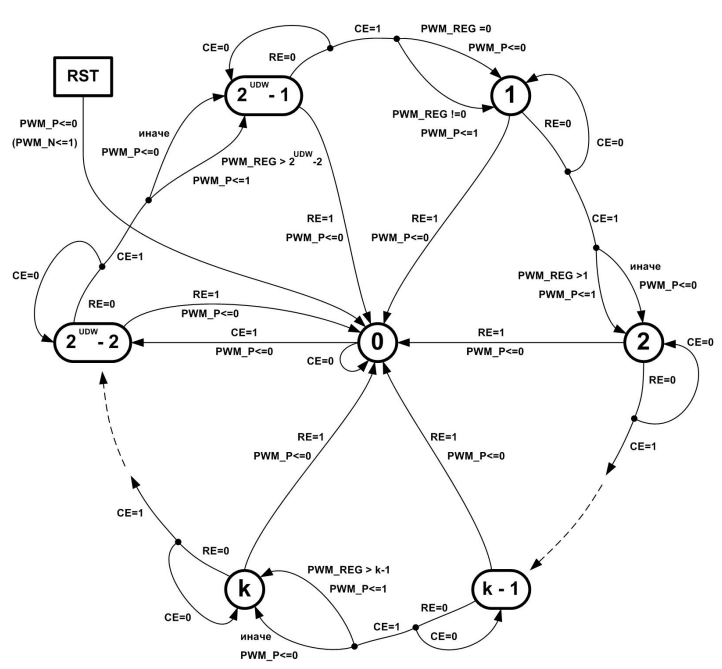
\includegraphics[width=0.55\linewidth]{course-plis/images/lab4/graph}
	\caption{Граф переходов конечного автомата}
	\label{fig:5graph}
\end{figure}

Входной регистр позволяет закончить период генерации ШИМ-сигнала на
основе неизменной управляющей комбинации, зафиксированной перед
началом текущего периода. 

Период генерации начинается в состоянии $2UDW - 1$ и заканчивается в состоянии $2UDW - 2$. Таким образом, изменения
комбинации на входе PWM\_IN не приведут к искажению формы выходного
сигнала.

Вход синхронного сброса RE предназначен для возврата автомата в
исходное состояние --- 0 и для перевода выходов в пассивное состояние.
Синхронный сброс является приоритетной операцией и воздействует
независимо от разрешения синхронизации CE. 

На входной регистр
PWM\_REG синхронный сброс не оказывает воздействия.
Временная диаграмма начала цикла работы генератора после синхронного
сброса показана на Рисунке~\ref{fig:sync-rst}. 

\begin{figure}[h!]
	\centering
	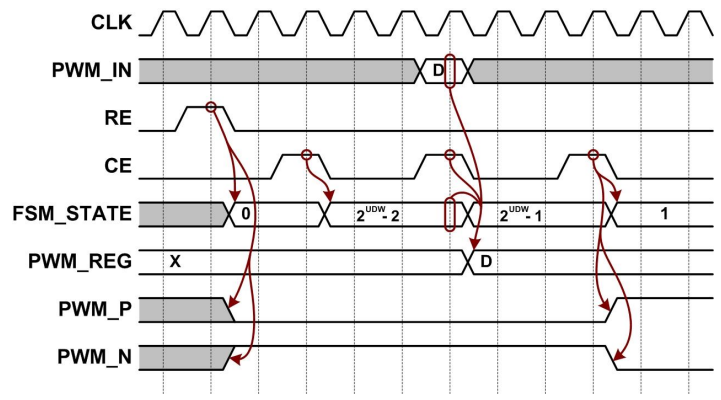
\includegraphics[width=0.54\linewidth]{course-plis/images/lab4/sync-rst}
	\caption{Синхронный сброс генератора}
	\label{fig:sync-rst}
\end{figure}




\section{Создание проекта САПР Xilinx ISE}
В ходе выполнения данного задания была реализована модель цифрового узла. Функциональная схема генератора ШИМ-сигналов приведена на Рисунке~\ref{fig:func-scheme}.

\begin{figure}[h!]
	\centering
	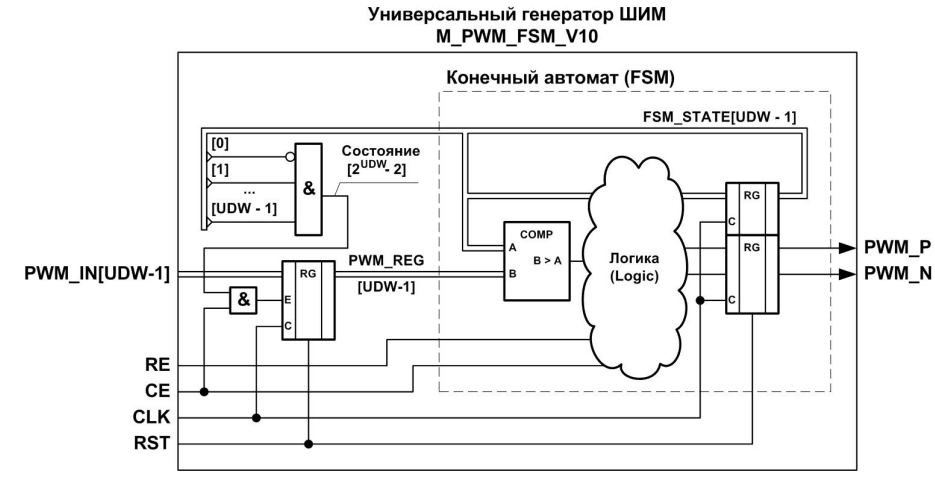
\includegraphics[width=0.65\linewidth]{course-plis/images/lab4/func-scheme}
	\caption{Функциональная схема генератора}
	\label{fig:func-scheme}
\end{figure}

Перечислим функциональные узлы, которые уже были реализованы ранее. 

\begin{enumerate}
	\item Делитель частоты. Реализован в разделе~\ref{cha:lab2}.
	\item Фильтр дребезга кнопок. Реализован в разделе~\ref{cha:lab2}.
	\item Конечный автомат генератор последовательности. Реализован в разделе~\ref{cha:lab2}.
	\item Блок управления матричным индикатором. Реализован в разделе~\ref{cha:lab4}.
\end{enumerate}

\paragraph{ШИМ генератор.}
Был описан модуль на языке программирования Verilog, реализующий ШИМ генератор. 
Исходный код данного функционального блока приведен в Приложении~\ref{cha:appendix1} в Листинге~\ref{lst:5pwm}.


\paragraph{Сдвиговый регистр.}
На языке программирования Verilog был описан 64-разрядный сдвиговый регистр, оформленный в виде модуля. Данный модуль реализует две операции:
\begin{enumerate}
	\item Циклический сдвиг влево на 4 разряда.
	\item Циклический сдвиг вправо на 4 разряда
\end{enumerate}

Исходный код данного функционального блока приведен в Приложении~\ref{cha:appendix1} в Листинге~\ref{lst:5shift}.

\paragraph{Блок управления матричным индикатором.}
Изменим модуль, реализующий блок управления матричным индикатором --- установим новый способ отображения входных сигналов на дисплей согласно Рисунку~\ref{fig:display-out}.

\begin{lstlisting}[caption={Измененный способ коммутации}]
	always@*
	begin
		rows = {data[63-column_ctr],
				data[55-column_ctr],
				data[47-column_ctr],
				data[39-column_ctr],
				data[31-column_ctr],
				data[23-column_ctr],
				data[15-column_ctr],
				data[7-column_ctr]
				};
	end
\end{lstlisting}

Исходный код данного функционального блока приведен в Приложении~\ref{cha:appendix1} в Листинге~\ref{lst:5lcd}.

\paragraph{Модуль верхнего уровня.}
В ходе выполнения данного задания был реализован модуль верхнего уровня на языке Verilog.
Исходный код данного модуля приведен в Приложении~\ref{cha:appendix1} на Листинге~\ref{lst:5top}.

\paragraph{Тестовый модуль.}
Опишем процесс создания модуля, который будет организовывать тестовое окружение рассматриваемой части цифрового логического устройства. 
В модуле верхнего уровня описан генератор тактового сигнала частотой 48 МГц, который используется в качестве тактового сигнала для всех синхронных функциональных узлов в составе устройства. 

Сигнал с частотой 1МГц будет используется как сигнал разрешения счета для генераторов ШИМ-сигналов, счетчика столбцов.

Исходный код данного модуля приведен в Приложении~\ref{cha:appendix1} в Листинге~\ref{lst:5test-top}.


\section{Тестирование и отладка средствами симулятора ISim}
После компоновки проекта, подключения модуля верхнего уровня, была проведена верификация спроектированных моделей с помощью симулятора iSim из состава САПР Xilinx ISE Design Suite. Результаты тестирования можно видеть в Приложении~\ref{cha:appendix2} на Рисунках~\ref{fig:5isim1}.~\ref{fig:5isim2}.





\section{Вывод}

В данном разделе нами были получены общие навыки работы с программным обеспечением Xilinx ISE Design Suite, изучены основы языка Verilog.

С помощью полученных знаний был спроектирован функциональный узел--генератор ШИМ сигналов, который был использован для управления светодиодными индикаторами, а также 64-рязрядный сдвиговый регистр.



\clearpage

%\cite{d2004mysql},\cite{baldinLatex}, \cite{converse2004php5}, \cite{yurt2011dev}.

\backmatter %% Здесь заканчивается нумерованная часть документа и начинаются ссылки и
            %% заключение

\Conclusion % заключение к отчёту

Результатом работы над данной курсовой работой является ознакомление с проблематикой разработки мультисинхронных устройств, реализация цифрового устройства ресинхронизации данных, представляющего собой асинхронную очередь данных, тактируемого двумя независимыми синхросигналами.

В ходе данной работы были проведены мероприятия по разработке функциональной и структурной схемы цифрового устройства и устройств, необходимых для его работы; созданию модуля, реализующего устройство ресинхронизации данных на языке описания аппаратуры Verilog; включению данного устройства в состав сложных устройств и проведение его отладки и тестирования.

Цели и задачи по реализации устройства для ресинхронизации данных выполнены. 

%%% Local Variables: 
%%% mode: latex
%%% TeX-master: "rpz"
%%% End: 


% % Список литературы при помощи BibTeX
% Юзать так:
%
% pdflatex rpz
% bibtex rpz
% pdflatex rpz

\bibliographystyle{gost780u}
\bibliography{course-plis/rpz}

%%% Local Variables: 
%%% mode: latex
%%% TeX-master: "rpz"
%%% End: 


%\cite{tarasov2011},\cite{goncharovskyMaj}. \cite{ushenina}.\cite{hata2012fpga}, \cite{cummings2002simulation},, \cite{stempcovsky},\cite{harris}



%
\begin{appendixes}
	Приложение \ref{cha:appendix1} ---  листинги реализованных модулей
	
	Приложение \ref{cha:appendix2} --- результаты симуляции и тестирования модулей
\end{appendixes}

\clearpage
\appendix   % Тут идут приложения
%\setcounter{page}{24}
\fontsize{14}{16pt}\selectfont
\chapter{\\\hspace{-6mm}Листинг}
\label{cha:appendix1}

%Lab1
\captionof{lstlisting}{Реализация функций на вентильном уровне}
\lstinputlisting[label=lst:1mknf]{course-plis/scripts/mknf.v}


\captionof{lstlisting}{Реализация функций на поведенческом уровне}
\lstinputlisting[label=lst:1beh]{course-plis/scripts/behaviour.v}


\captionof{lstlisting}{Реализация логических функций. Файл верхнего уровня}
\lstinputlisting[label=lst:1top]{course-plis/scripts/top.v}


%Lab2

\captionof{lstlisting}{Цифровой автомат}
\lstinputlisting[label=lst:2fsm]{course-plis/scripts/fsm.v}

\captionof{lstlisting}{Делитель частоты}
\lstinputlisting[label=lst:2freq-div]{course-plis/scripts/freq_div.v}

\captionof{lstlisting}{Фильтр дребезга}
\lstinputlisting[label=lst:2filter]{course-plis/scripts/m_btn_filter.v}

 
\captionof{lstlisting}{Тестирование цифрового автомата}
\lstinputlisting[label=lst:2fsm-test]{course-plis/scripts/test-fsm.v}

\captionof{lstlisting}{Цифровой автомат. Файл верхнего уровня}
\lstinputlisting[label=lst:2top]{course-plis/scripts/top2.v}



%Lab 3


\captionof{lstlisting}{Описание главного алгоритма}
\lstinputlisting[label=lst:3seq-auto]{course-plis/scripts/seqAuto.v}


\captionof{lstlisting}{Описание модуля работы с семисегментыми индикаторами алгоритма}
\lstinputlisting[label=lst:3display]{course-plis/scripts/NexysDisplay.v}

%\captionof{lstlisting}{Описание вектор--функции}
%\lstinputlisting[label=lst:3func]{course-plis/scripts/outFunc.v}

\captionof{lstlisting}{Описание сигнального дешифратора}
\lstinputlisting[label=lst:3decode]{course-plis/scripts/SevenSegDec.v}

\captionof{lstlisting}{Реализация анализатора последовательности. Файл верхнего уровня}
\lstinputlisting[label=lst:3top]{course-plis/scripts/top.v}


%Lab4

\captionof{lstlisting}{Описание блока управления матричным индикатором}
\lstinputlisting[label=lst:4lcd]{course-plis/scripts/LCDMatrixDirver.v}

\captionof{lstlisting}{Управление матричным индикатором. Модуль вернхнего уровня}
\lstinputlisting[label=lst:4top]{course-plis/scripts/4top.v}


\captionof{lstlisting}{Управление матричным индикатором. Тестовый модуль}
\lstinputlisting[label=lst:4test-top]{course-plis/scripts/4test_top.v}


%Lab5
\captionof{lstlisting}{Генератор ШИМ}
\lstinputlisting[label=lst:5pwm]{course-plis/scripts/lab5/pwm_m.v}

\captionof{lstlisting}{Сдвиговый регистр}
\lstinputlisting[label=lst:5shift]{course-plis/scripts/lab5/SR64_S4B.v}


\captionof{lstlisting}{Блок управления матричным индикатором}
\lstinputlisting[label=lst:5lcd]{course-plis/scripts/lab5/LCDM_new.v}


\captionof{lstlisting}{Генератор ШИМ. Модуль верхнего уровня}
\lstinputlisting[label=lst:5top]{course-plis/scripts/lab5/top.v}


\captionof{lstlisting}{Генератор ШИМ. Тестовый модуль}
\lstinputlisting[label=lst:5test-top]{course-plis/scripts/lab5/test_top.v}



%\begin{lstlisting}[style=pseudocode,caption={Алгоритм оценки дипломных работ}]
%	sdfsadf sdf asdf sadf s
%\end{lstlisting}
%%% Local Variables: 
%%% mode: latex
%%% TeX-master: "rpz"
%%% End: 

\clearpage
\fontsize{14}{16pt}\selectfont
%\chapter{\\\hspace{-6mm}Результаты симуляции}
\chapter{Результаты симуляций}
\label{cha:appendix2}

%Lab1
\begin{figure}[h!]
	\centering
	\includegraphics[width=\linewidth]{course-plis/images/lab1/isim}
	\caption{Реализация комбинационной логической схемы}
	\label{fig:1isim}
\end{figure}


%Lab2

% TODO: \usepackage{graphicx} required
\begin{figure}[h!]
	\centering
	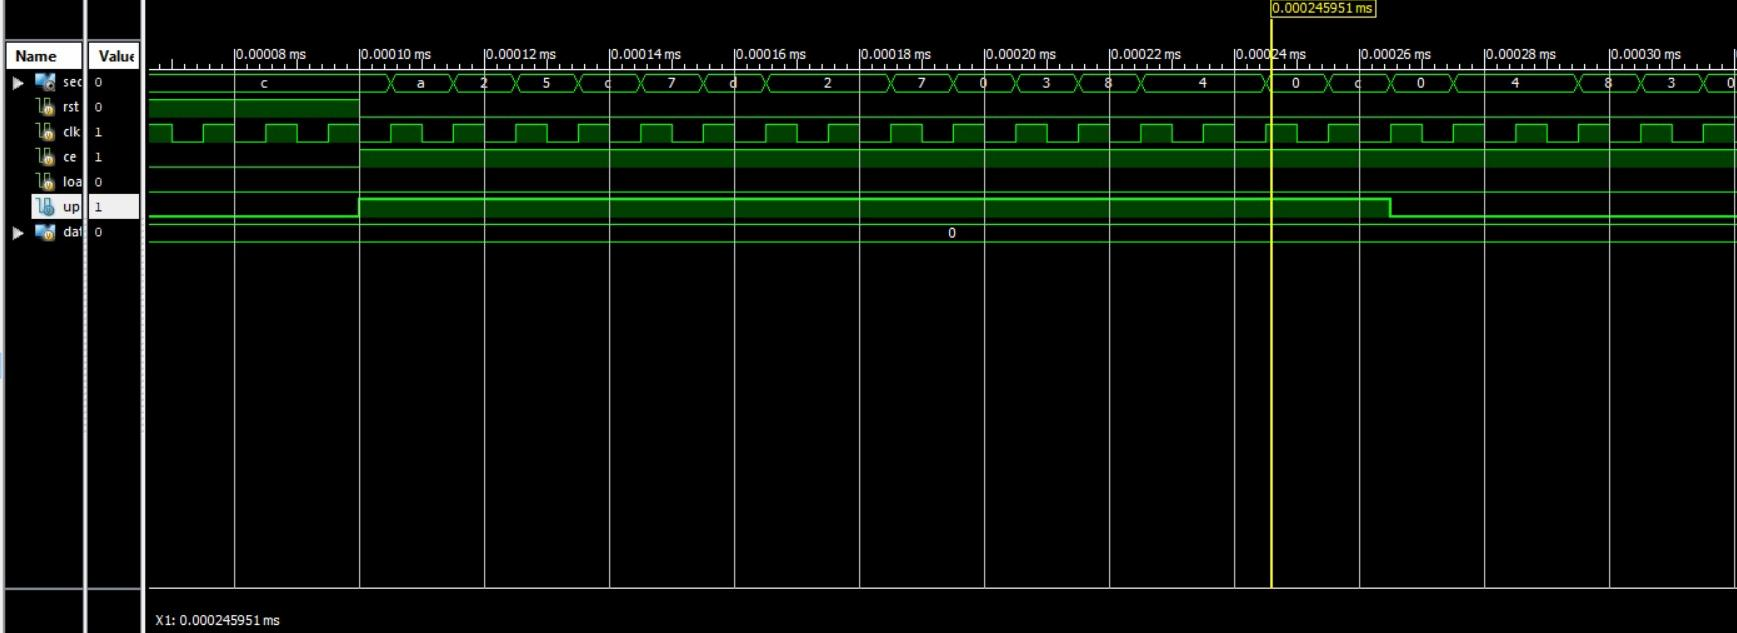
\includegraphics[width=\linewidth]{course-plis/images/lab2/test-result2.1}
	\caption{Реализация цифрового автомата. Часть 1}
	\label{fig:2isim1}
\end{figure}

\begin{figure}[h!]
	\centering
	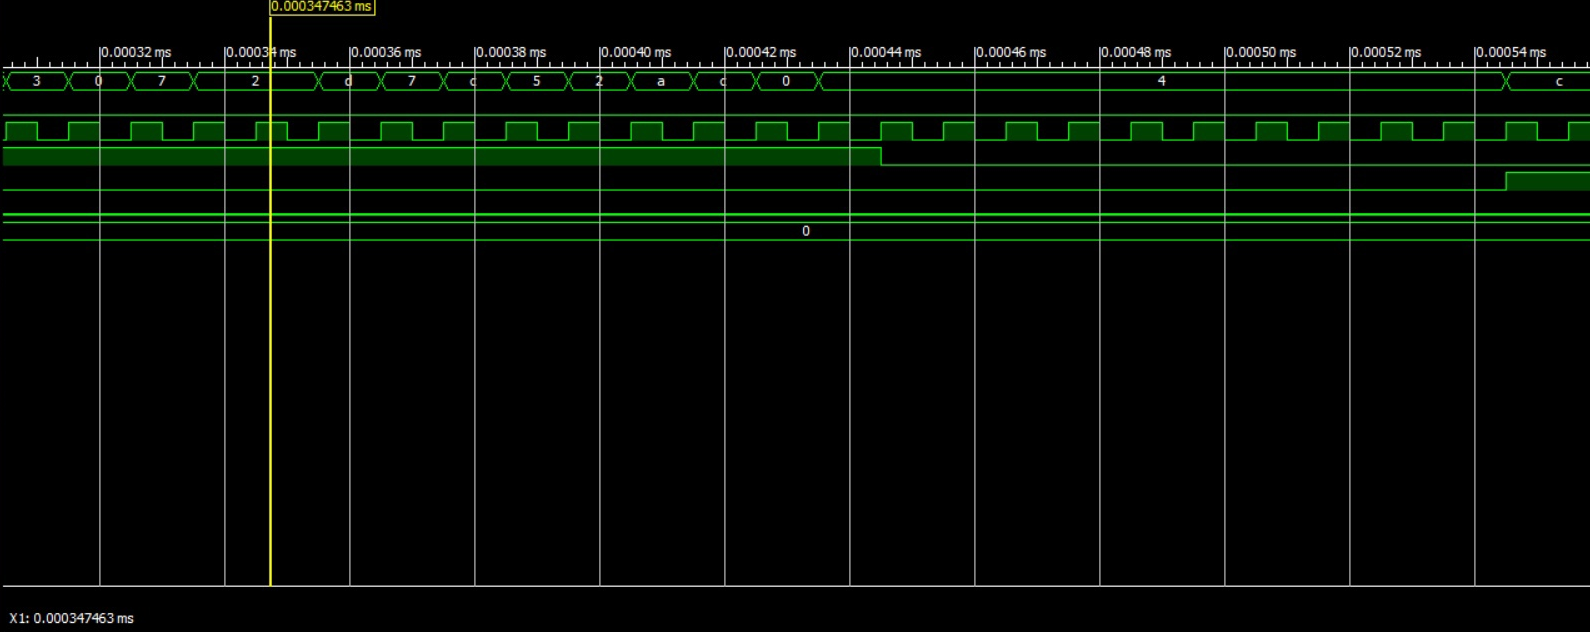
\includegraphics[width=\linewidth]{course-plis/images/lab2/test-result2.3}
	\caption{Реализация цифрового автомата. Часть 2}
	\label{fig:2isim2}
\end{figure}





% Lab3 

% TODO: \usepackage{graphicx} required
\begin{figure}[h!]
	\centering
	\includegraphics[width=1\linewidth]{course-plis/images/lab3/page-1}
	\caption{Реализация анализатора последовательности. Часть 1}
	\label{fig:3page-1}
\end{figure}
% TODO: \usepackage{graphicx} required
\begin{figure}[h!]
	\includegraphics[width=1\linewidth]{course-plis/images/lab3/page-2}
\caption{Реализация анализатора последовательности. Часть 2}
	\label{fig:3page-2}
\end{figure}
% TODO: \usepackage{graphicx} required
%\begin{figure}[h!]
%	\centering
%	\includegraphics[width=1\linewidth]{course-plis/images/lab3/page-3}
%	\caption{Реализация анализатора последовательности. Часть 3}
%	\label{fig:3page-3}
%\end{figure}
% TODO: \usepackage{graphicx} required
\begin{figure}[h!]
	\centering
	\includegraphics[width=1\linewidth]{course-plis/images/lab3/page-4}
	\caption{Реализация анализатора последовательности. Часть 3}
	\label{fig:3page-4}
\end{figure}
% TODO: \usepackage{graphicx} required
\begin{figure}[h!]
	\centering
	\includegraphics[width=1\linewidth]{course-plis/images/lab3/page-5}
	\caption{Реализация анализатора последовательности. Часть 4}
	\label{fig:3page-5}
\end{figure}
% TODO: \usepackage{graphicx} required
\begin{figure}[h!]
	\centering
	\includegraphics[width=1\linewidth]{course-plis/images/lab3/page-6}
	\caption{Реализация анализатора последовательности. Часть 5}
	\label{fig:3page-6}
\end{figure}



%Lab 4
\begin{figure}[h!]
	\centering
	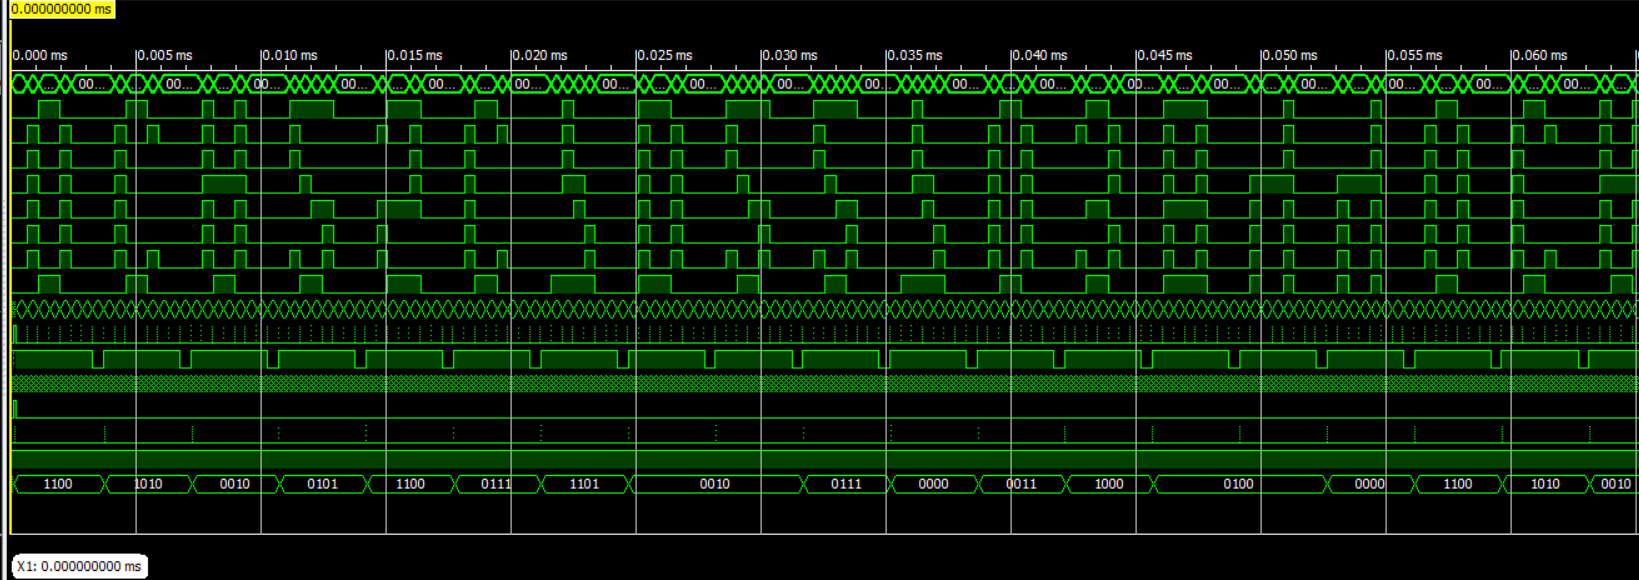
\includegraphics[width=1\linewidth]{course-plis/images/lab4/4isim}
	\caption{Управление матричным индикатором. Результат симуляции}
	\label{fig:4isim}
\end{figure}



%Lab5
\begin{figure}[h!]
	\centering
	\includegraphics[width=1\linewidth]{course-plis/images/lab5/isim1}
	\caption{Генерация ШИМ. Результат симуляции. Часть 1}
	\label{fig:5isim1}
\end{figure}

\begin{figure}[t!]
	\centering
	\includegraphics[width=1\linewidth]{course-plis/images/lab5/isim2}
	\caption{Генерация ШИМ. Результат симуляции. Часть 2}
	\label{fig:5isim2}
\end{figure}

%\vspace{50ex}
%\vfill




%\begin{lstlisting}[style=pseudocode,caption={Алгоритм оценки дипломных работ}]
%	sdfsadf sdf asdf sadf s
%\end{lstlisting}
%%% Local Variables: 
%%% mode: latex
%%% TeX-master: "rpz"
%%% End: 

\clearpage
%%\chapter{\\\hspace{-6mm}Руководство пользователя}
\label{cha:appendix3}
\setlength{\parindent}{12.5mm}

В данном приложении приведены правила использования цифрового устройства по ресинхронизации данных. 

Чтобы использовать аппаратный блок, спроектированный в ходе данной курсовой работы, в своих проектах, необходимо обратиться к списку выходов и входов, приведенному в разделе \ref{sec:design} настоящей курсовой работы и подключить модуль соответствующим образом.

Следует помнить, что данные на выход подаются по мере образования во входном буфере не менее четырех восьмиразрядных слов. Тактовые сигналы входного и выходного каналов независимы, однако тактовая частота для выхода устройства должна составлять как минимум  четверть от тактовой частоты входного интерфейса устройства.

Восьмиразрядные числа, переданные на вход, образуют тридцатидвухразрядную выходную последовательность в прямом порядке следования битов (big endian). 

Следует обратить внимание, что устройство осуществляет контроль записи и чтения --- сигнализирует о пустоте или заполненности внутренней памяти, но не блокирует запись или чтение самостоятельно. Управлять разрешением на запись и чтение должны внешние узлы. Схема лишь не допускает обращения к одному участку памяти для записи и чтения единовременно.

Устройство не поддерживает сброс внутренней памяти, так как обычно память в устройствах, реализуемых на ПЛИС представлена в виде блочной оперативной памяти и выделенной оперативной памяти. Эти ресурсы обычно не поддерживают сброс. Сброс возможно реализовать в регистрах. 


%\begin{lstlisting}[style=pseudocode,caption={Алгоритм оценки дипломных работ}]
%	sdfsadf sdf asdf sadf s
%\end{lstlisting}
%%% Local Variables: 
%%% mode: latex
%%% TeX-master: "rpz"
%%% End: 

%\clearpage
%\chapter{Еще картинки}
\label{cha:appendix2}

\begin{figure}
\centering
\caption{Еще одна картинка, ничем не лучше предыдущей. Но надо же как-то заполнить место.}
\end{figure}

%%% Local Variables: 
%%% mode: latex
%%% TeX-master: "rpz"
%%% End: 





\end{document}

%%% Local Variables:
%%% mode: latex
%%% TeX-master: t
%%% End:
